\documentclass[conference]{IEEEtran}
\usepackage{cite}
\usepackage{amsmath,amssymb,amsfonts}
\usepackage{algorithmic}
\usepackage{graphicx}
\usepackage{textcomp}
\usepackage{xcolor}
\def\BibTeX{{\rm B\kern-.05em{\sc i\kern-.025em b}\kern-.08em
    T\kern-.1667em\lower.7ex\hbox{E}\kern-.125emX}}
\begin{document}

\title{Recurrent networks recognize patterns with low-dimensional oscillations}

\author{\IEEEauthorblockN{1\textsuperscript{st} Keith T. Murray}
\IEEEauthorblockA{\textit{Department of Brain and Cognitive Sciences} \\
\textit{Massachusetts Institute of Technology}\\
Cambridge, USA \\
ktmurray@mit.edu}
}

\maketitle

\begin{abstract}
This study proposes a novel dynamical mechanism for pattern recognition discovered by interpreting a recurrent neural network (RNN) trained on a simple task inspired by the SET card game. We interpreted the trained RNN as recognizing patterns via phase shifts in a low-dimensional limit cycle in a manner analogous to transitions in a finite state automaton (FSA). We further validated this interpretation by handcrafting a simple oscillatory model that reproduces the dynamics of the trained RNN. Our findings not only suggest of a potential dynamical mechanism capable of pattern recognition, but also suggest of a potential neural implementation of FSA. Above all, this work contributes to the growing discourse on deep learning model interpretability.
\end{abstract}

\begin{IEEEkeywords}
Pattern recognition, Recurrent neural networks, Neural dynamics, Cognitive modeling, Deep learning interpretability
\end{IEEEkeywords}

\section{Introduction}
Pattern recognition is fundamental to human cognition, influencing perception, language, and reasoning\cite{inhelder1964early}. Despite substantial advances in machine learning algorithms and models\cite{bishop2006pattern,lecun2015deep}, understanding the computational and neurological foundations of pattern recognition in human cognition remains a challenge. Recent studies applying recurrent neural networks (RNNs) to neural and cognitive modeling have led to the development of a variety of theories concerning the potential dynamical mechanisms responsible for various cognitive abilities \cite{sussillo2013opening,mante2013context,driscoll2022flexible,kay2022neural,pals2023trained}. This study builds on this research direction and these findings by proposing a simple pattern recognition task---inspired by the SET card game---solved by an RNN through phase shifts in a low-dimensional limit cycle. We theorize that this learned dynamical mechanism parallels transitions in a finite state automaton (FSA), suggesting a potential neural implementation of FSAs. To support this theory, we handcrafted a simple oscillatory model based on our interpretation that emulates the trained RNN's low-dimensional dynamics. Our findings not only add to the current research direction of purposing dynamical mechanisms underlying cognition, but also provide insights into deep learning model interpretability.

\section{Background}

\subsection{Dynamical motifs in RNNs}

Previous work by \cite{driscoll2022flexible} showed that RNNs trained on many cognitive tasks learned a series of modular, low-dimensional, dynamical phenomena (e.g. attractors, limit cycles, bifurcations \cite{strogatz2018nonlinear}), termed \textit{dynamical motifs}, that were shared among all cognitive tasks. In addition, simple tasks would learn simple dynamical motifs and complex tasks would combine multiple of these motifs in a manner apt for performing in the complex task. This work suggests that all cognitive abilities have associated simple dynamical phenomena that are implemented at the neural level. It is possible that the brain only implements a handful of simple dynamical motifs that can be combined and reused to perform all cognitive tasks.

\subsection{Dynamical mechanisms for transitive inference}

Previous work by \cite{kay2022neural} showed that RNNs trained to perform a transitive inference task learned a simple dynamical mechanism characterized by a single oscillation and a collinear encoding of stimulus inputs. To perform transitive inference, the RNN would encode stimuli as a linear input into the dynamical mechanism and the oscillatory activity of the mechanism would subtract the magnitude of subsequent encoded stimuli. Ref. \cite{kay2022neural} hypothesized that cognitive abilities requiring transitive inference might incorporate this particular dynamical mechanism. Building on this interpretation and motivation, we sought to uncover a potential dynamical mechanism underlying pattern recognition through training RNNs and interpreting their learned dynamics.

\subsection{Why do interpretable dynamical mechanisms emerge?}
\label{interpretablemotifs}

The simplicity of the dynamical mechanisms learned in \cite{driscoll2022flexible} and \cite{kay2022neural} is initially surprising; however, both studies incorporated substantial regularizations during the training of RNNs that biased the learned dynamics to be low-dimensional and interpretable. These regularizations were an L2 regularization of the trainable weights and the recurrent activations of the RNN. These constraints are well known to produce interpretable dynamics in RNNs and have a potential biophysical interpretations. Regularizations on the trainable weights reflect a synaptic resource constraint and regularizations on the recurrent activations reflect a cellular metabolic constraint\cite{sussillo2015neural,cueva2018emergence}. In this work, we used these regularizations in order to bias our model to learn an interpretable dynamical mechanism.

\section{Methodology}
Our methodology is divided into three parts: defining our novel pattern recognition task (sec.~\ref{taskmethod}), defining the model and its parameters (sec.~\ref{ctrnnmodel}), and describing our analysis methods (sec.~\ref{analysismodel}).

\subsection{Task}
\label{taskmethod}

While there exists a host of pattern recognition and classification tasks in the machine learning community\cite{bishop2006pattern,lecun2015deep}, their associated datasets may be too complex and/or noisy to elicit interpretable dynamical mechanisms. We instead took inspiration for the design of our own task from the card game SET \cite{gordon2017joy}. SET is a card game where players try to identify sets of three cards out of a field of 12 cards. Each card has four attributes: shape, color, number, and shading. Each of these attributes has three possible values. A valid set is found when for each attribute, all the values pertaining to that attribute across all 3 cards are the \textit{same} or \textit{different}. While the patterns in SET appear to be simple, the game is regarded as being cognitively demanding\cite{gordon2017joy}.

While the complete game of SET involves searching through 12 cards, each with four attributes, our task was simplified to only concern classifying three cards, with one attribute each, as a valid set. We refer to this attribute as \textit{color} and the three values associated as \textit{green}, \textit{purple}, and \textit{red}. The task involved sequentially presenting three colors to an agent and tasking the agent with classifying if the colors presented constituted a valid set (i.e. the agent decides if all the colors presented were the \textit{same} or \textit{different}).

All trials of the task were $500 ms$. There was a delay period of $30 ms$ at the beginning and $100 ms$ at the end of the trial where no colors were presented. A color was presented for $20 ms$, and there was at least a $30 ms$ gap between the presentation of colors (Fig.~\ref{trial}). Given that our agent was an RNN, each color was encoded as a $100$-dimensional vector\footnote{Our use of a $100$-dimensional vector was inspired by \cite{kay2022neural}. This dimensionality ensured that stimulus representations were uncorrelated in the activity space of the model.} with values drawn from a Gaussian distribution\footnote{The same encoding vectors were used across all training and testing trials.}. The RNN was tasked with producing a value of $+1$ to indicate a valid set or $-1$ to indicate an invalid set at the end of a trial.

\begin{figure}[htbp]
\centerline{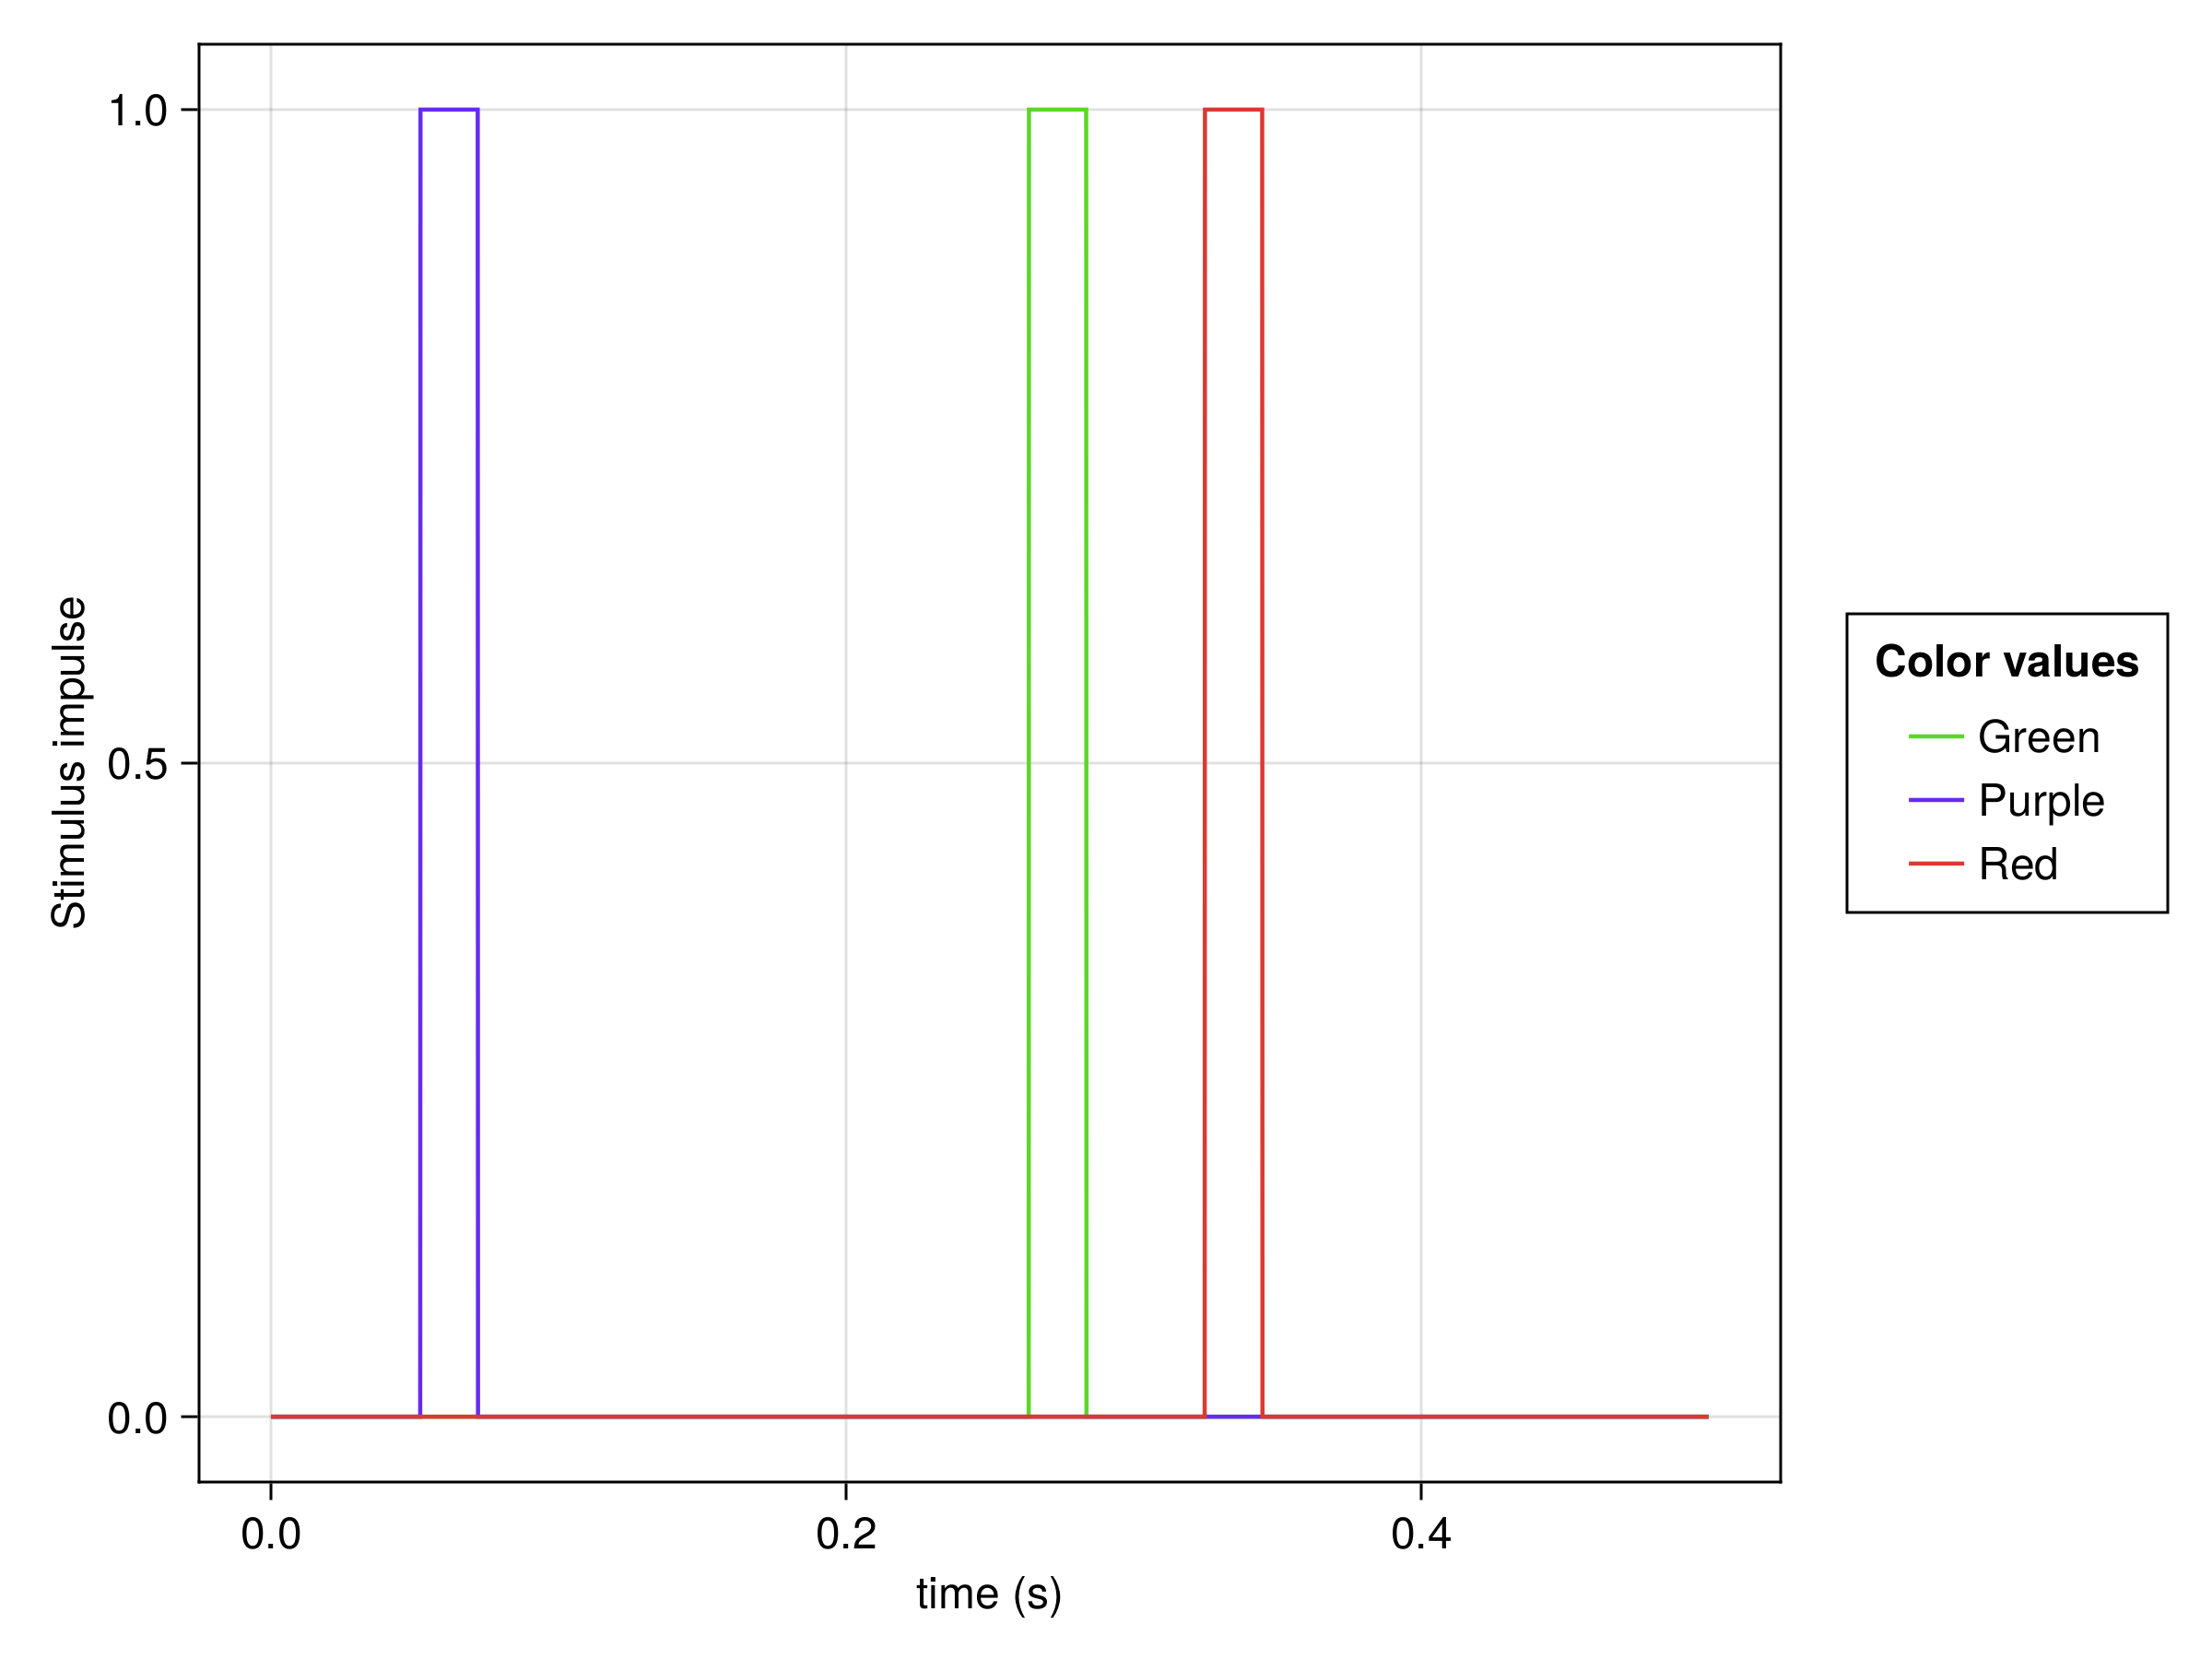
\includegraphics[scale=0.10]{example_trial.png}}
\caption{A sample trial showing the colors purple, green, and red being presented. This trial constitutes a valid set.}
\label{trial}
\end{figure}

The model was trained on a training dataset of $540$ trials. The proportion of accepting to rejecting trials in the training dataset was $50\%$. $27$ trails were generated for the testing dataset, where each trial consisted of a distinct combination of presented colors. Trials were mini-batched during training into batches of $108$ trials.

\subsection{Model}
\label{ctrnnmodel}

We describe our model according to the framework proposed in \cite{richards2019deep}.

\textbf{Architecture:} The model was a standard continuous-time RNN:
\begin{equation}
    \tau \dot{x}_i(t) = -x_i(t) + \sum^{N}_{k=1} J_{ik}r_k(t) + \sum^{N^{in}}_{k=1}B_{ik}u_k(t) + b_i + \eta_i(t)
\end{equation}
\begin{equation}
    r_i(t) = \tanh(x_i)
\end{equation}
\begin{equation}
    z(t) = \sum^{N}_{k=1}W_{k}r_k(t) + b_{out}
\end{equation}
$\tau$ is interpreted as the time constant for the RNN and was set to $10 ms$. $x_i(t)$ is interpreted as the average voltage value for the $i$th subpopulation of cortical neurons at time $t$. $N$ is the total number of subpopulations of cortical neurons and was set at $100$. $u_k(t)$ is interpreted as the input stimulus function conveying color values. $N^{in}$ is the number of input dimensions and was, as stated in section 3.1, set at $100$. $\eta_i(t)$ is a random value drawn from a Gaussian distribution, $\mathcal{N}(0,0.10)$. $r_i(t)$ is interpreted as the average firing rate value for the $i$th subpopulation of cortical neurons. The activation function that converts voltage to firing rate is the hyperbolic tangent (tanh). $z(t)$ is the value of the output neuron.

Equation (1) was approximated with Euler's method and a step size ($\Delta t$) of $10 ms$ for all trials. The entirety of our model was coded in Julia\cite{bezanson2017julia} using the Lux framework\cite{pal2022lux} and SciML ecosystem\cite{rackauckas2017differentialequations,rackauckas2020universal}.

\textbf{Learning algorithm:} We used the AdamW learning algorithm\cite{loshchilov2017decoupled} and reverse mode automatic differentiation to train the adjustable parameters that define our neural network: the initial state $\textbf{x}(t=0)$, recurrent matrix $\textbf{J}$, input matrix $\textbf{B}$, input bias vector $\textbf{b}$, internal weight matrix $\textbf{W}$, and output bias $b_{out}$.. The initial learning rate was set to $10^{-4}$. L2 regularization, as mentioned in sec.~\ref{interpretablemotifs}, was implemented as a weight decay regularization in the AdamW algorithm and was set to $10^{-4}$.

\textbf{Objective function:} We used a mean squared error (MSE) objective function to compare the observed $z(t)$ value to the expected $\hat{z}(t)$ value. The last $5$ time steps of the $500 ms$ trail were used for the MSE function. Metabolic regularization, as mentioned in sec.~\ref{interpretablemotifs}, was added to the objective function to bias the recurrent activations toward being low in amplitude. The full objection function was the following:
\begin{equation}
    \mathcal{L}(\hat{z},z,\textbf{r}) = \frac{1}{5}\sum_{t=T-5}^{T}(\hat{z}(t)-z(t))^2 + \lambda\frac{1}{TN} \sum_{t,i=1}^{T,N} r^2_i(t)\Delta t
\end{equation}
$T$ is the total number of time steps, $50$ for all trials. $\lambda$ is the metabolic penalty and was set to $10^{-4}$.

\subsection{Analysis}
\label{analysismodel}

To analyze the learned representations of our model, we primarily utilized Principal Component Analysis (PCA), a popular dimensionality reduction technique. PCA has been prevalently employed in previous RNN research for visualizing the low-dimensional dynamics of RNNs \cite{sussillo2013opening,mante2013context,driscoll2022flexible,kay2022neural}. We performed PCA on the firing rates of our model, $\textbf{r}(t)$, under the condition of no recurrent noise, i.e., $\eta_i(t)=0$.

It is essential to mention that PCA mainly discerns the correlations amongst the firing rates of our model, rather than identifying causal, mechanistic properties \cite{langdon2022latent}. To address this inherent limitation of PCA, we developed a simplified model of the low-dimensional rates within our network. This approach allows us to confirm the existence of the mechanisms suggested by the PCA analysis.

Our initial hypothesis postulated that PCA would reveal an underlying fixed-point network in the shape of a hexagon (Fig.~\ref{hypothesisFSA}). Drawing inspiration from the Hopfield network \cite{b27} and insights provided in \cite{chaisangmongkon2017computing}, we conceived this notion of a hexagonal fixed-point network.

\begin{figure}[htbp]
\centerline{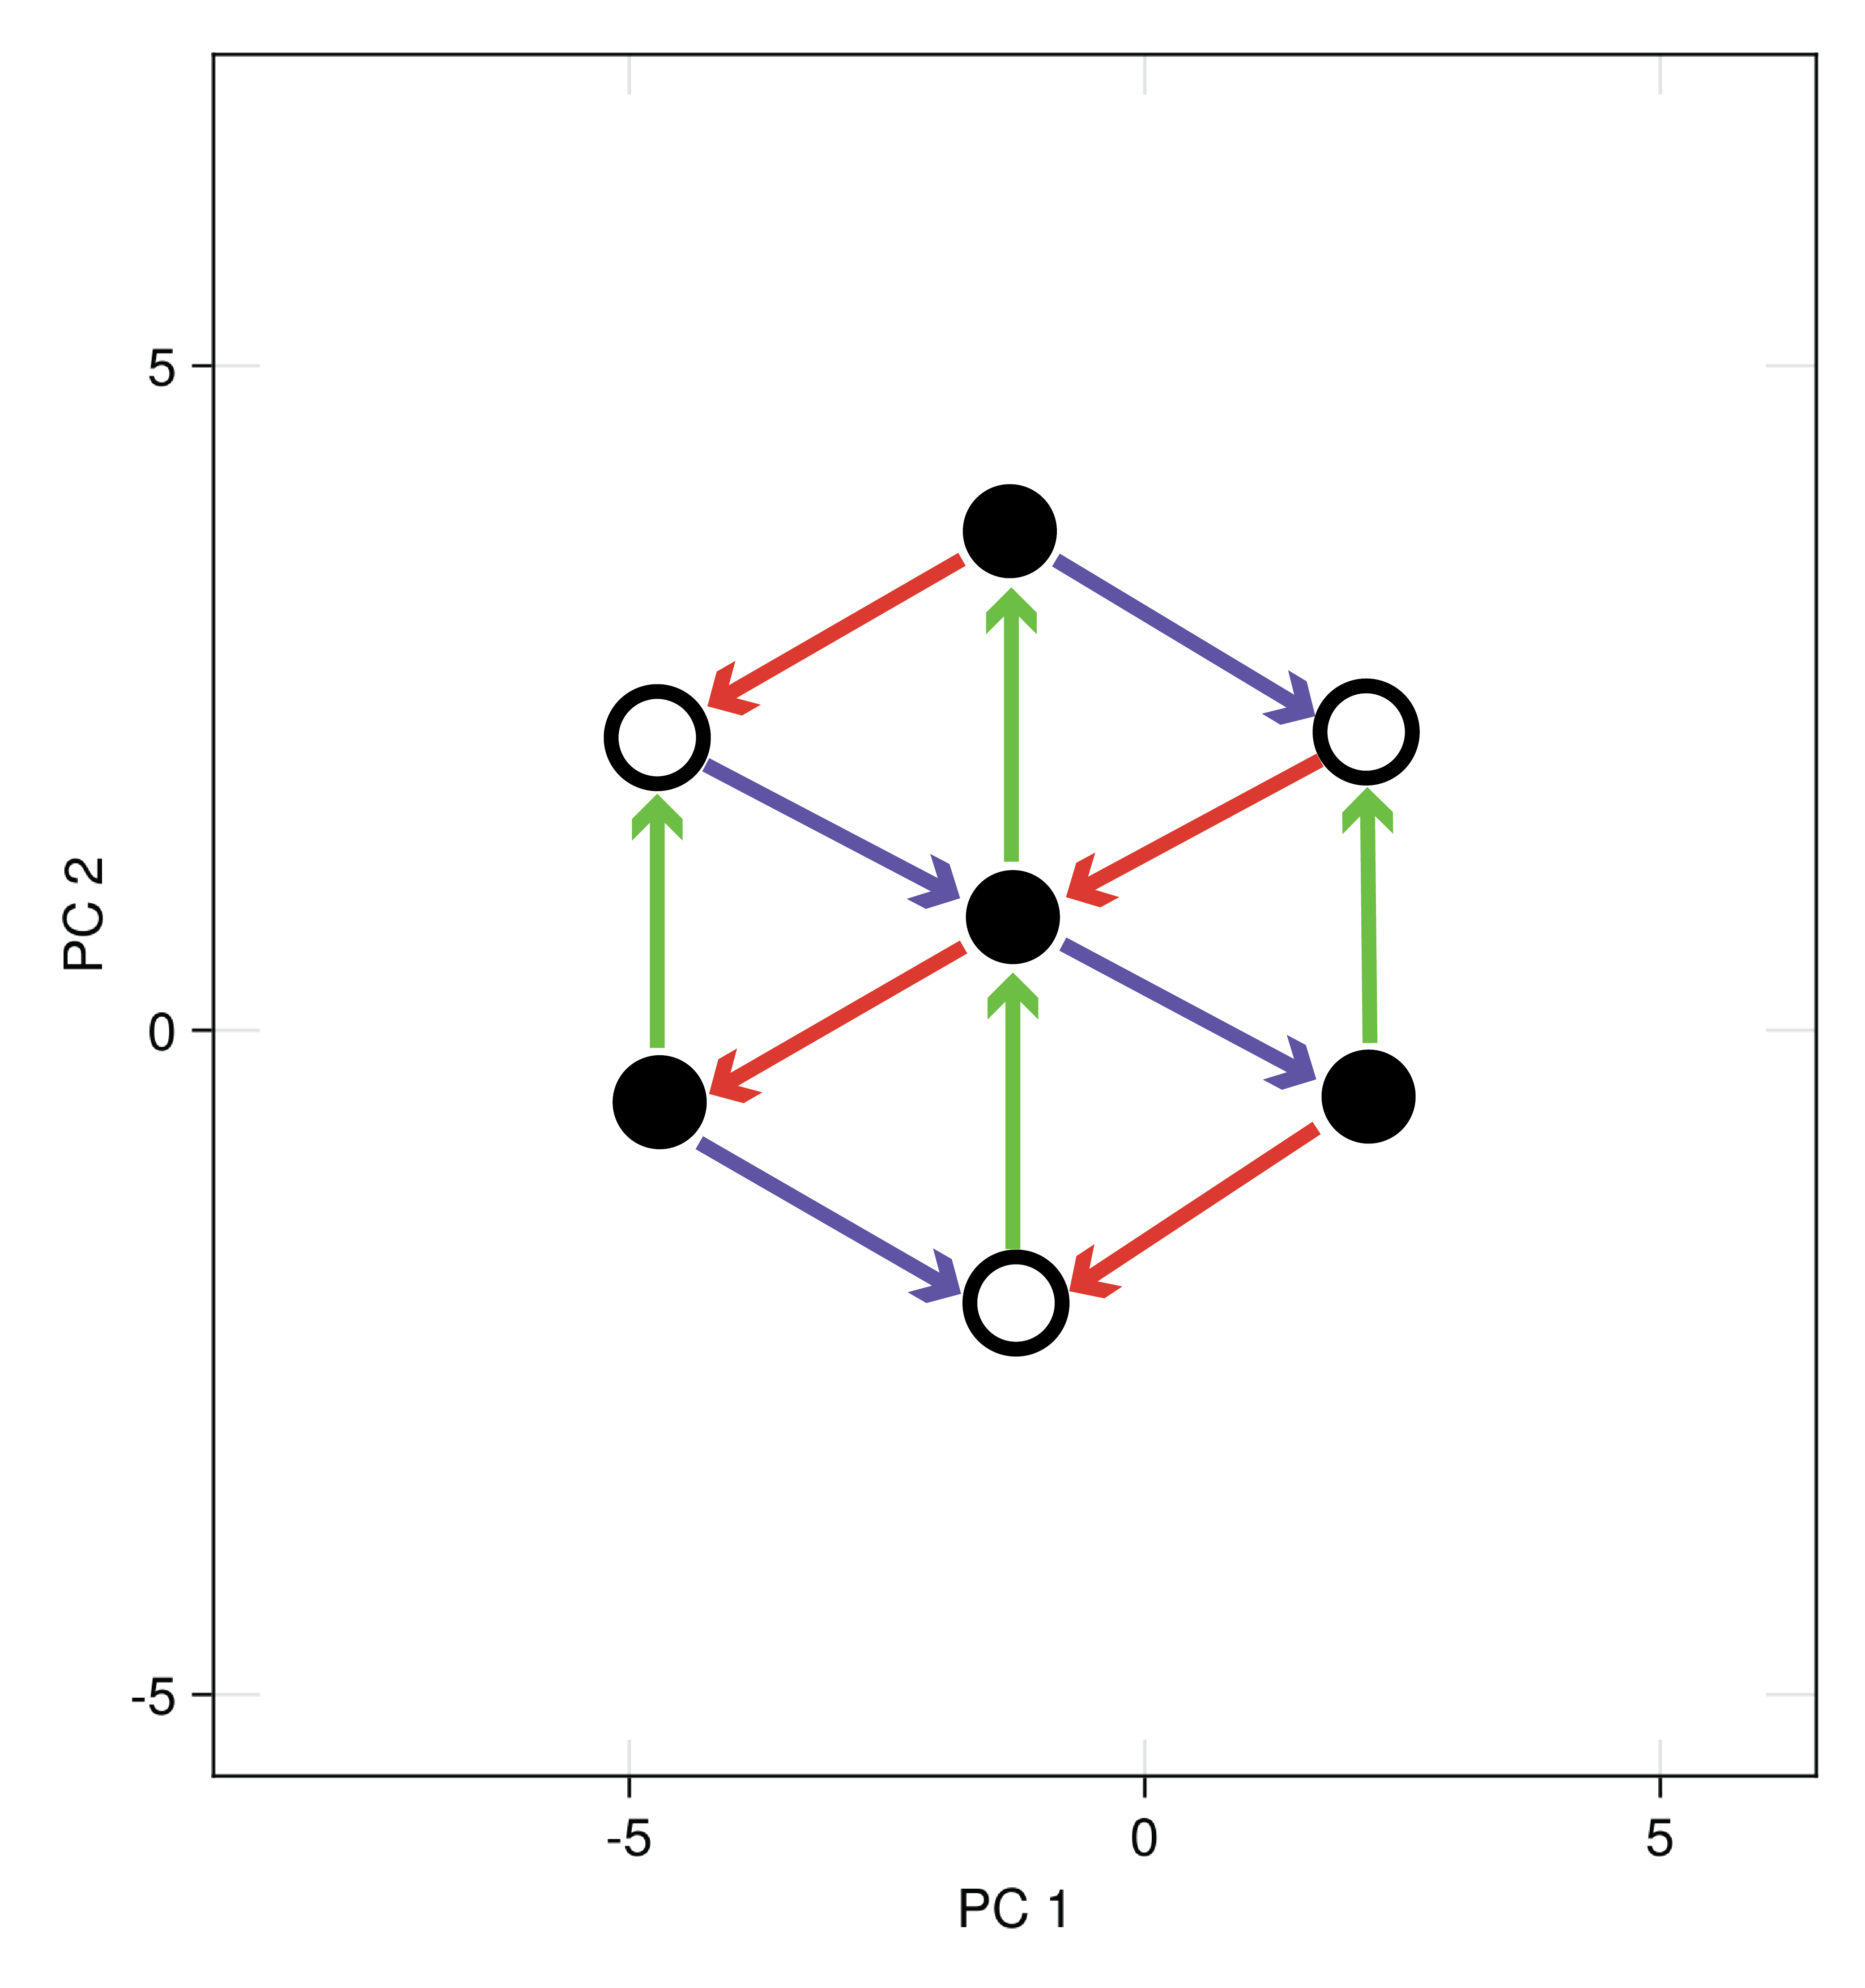
\includegraphics[scale=0.125]{hypothesis.png}}
\caption{An illustration of our hypothesized low-dimensional, learned representation in the form of a hexagonal fixed-point network. Filled fixed points represent accepted patterns, while empty ones denote rejected patterns. Note that all transitions triggered by a specific color stimulus maintain a consistent directionality. The architecture of this network allows for linear segregation of accepting and rejecting fixed points in PC 3, simplifying classification tasks.}
\label{hypothesisFSA}
\end{figure}

In this hypothesized network, activity originates in the center with the sequential introduction of a color stimulus sequentially propelling the network's activity from one fixed-point to another. Note the consistent directionality associated with each color in the graph. Color transitions absent from the diagram are represented as self-loops. In PC 3, the fixed-points corresponding to acceptance and rejection can be linearly segregated, simplifying the classification process.

This hexagonal fixed-point network can be represented as an FSA, with valid patterns represented as a subset of the regular language of the FSA \cite{tivno1998finite}.

\section{Results}

\subsection{Accuracy and Preliminary Analysis}

The fully-trained RNN model demonstrated robust performance, achieving an accuracy of $96.30\%$ in training and $100.00\%$ in testing. In the absence of recurrent noise, the model displayed flawless performance, reaching an accuracy of $100.00\%$ in both training and testing. Despite this perfect accuracy, it was somewhat anticipated due to the straightforward nature of the dataset. The model's output exhibited an oscillatory pattern, with \textit{perturbations} corresponding to the introduction of the stimulus (Fig.~\ref{exampletrialstimuli}).

\begin{figure}[htbp]
\centerline{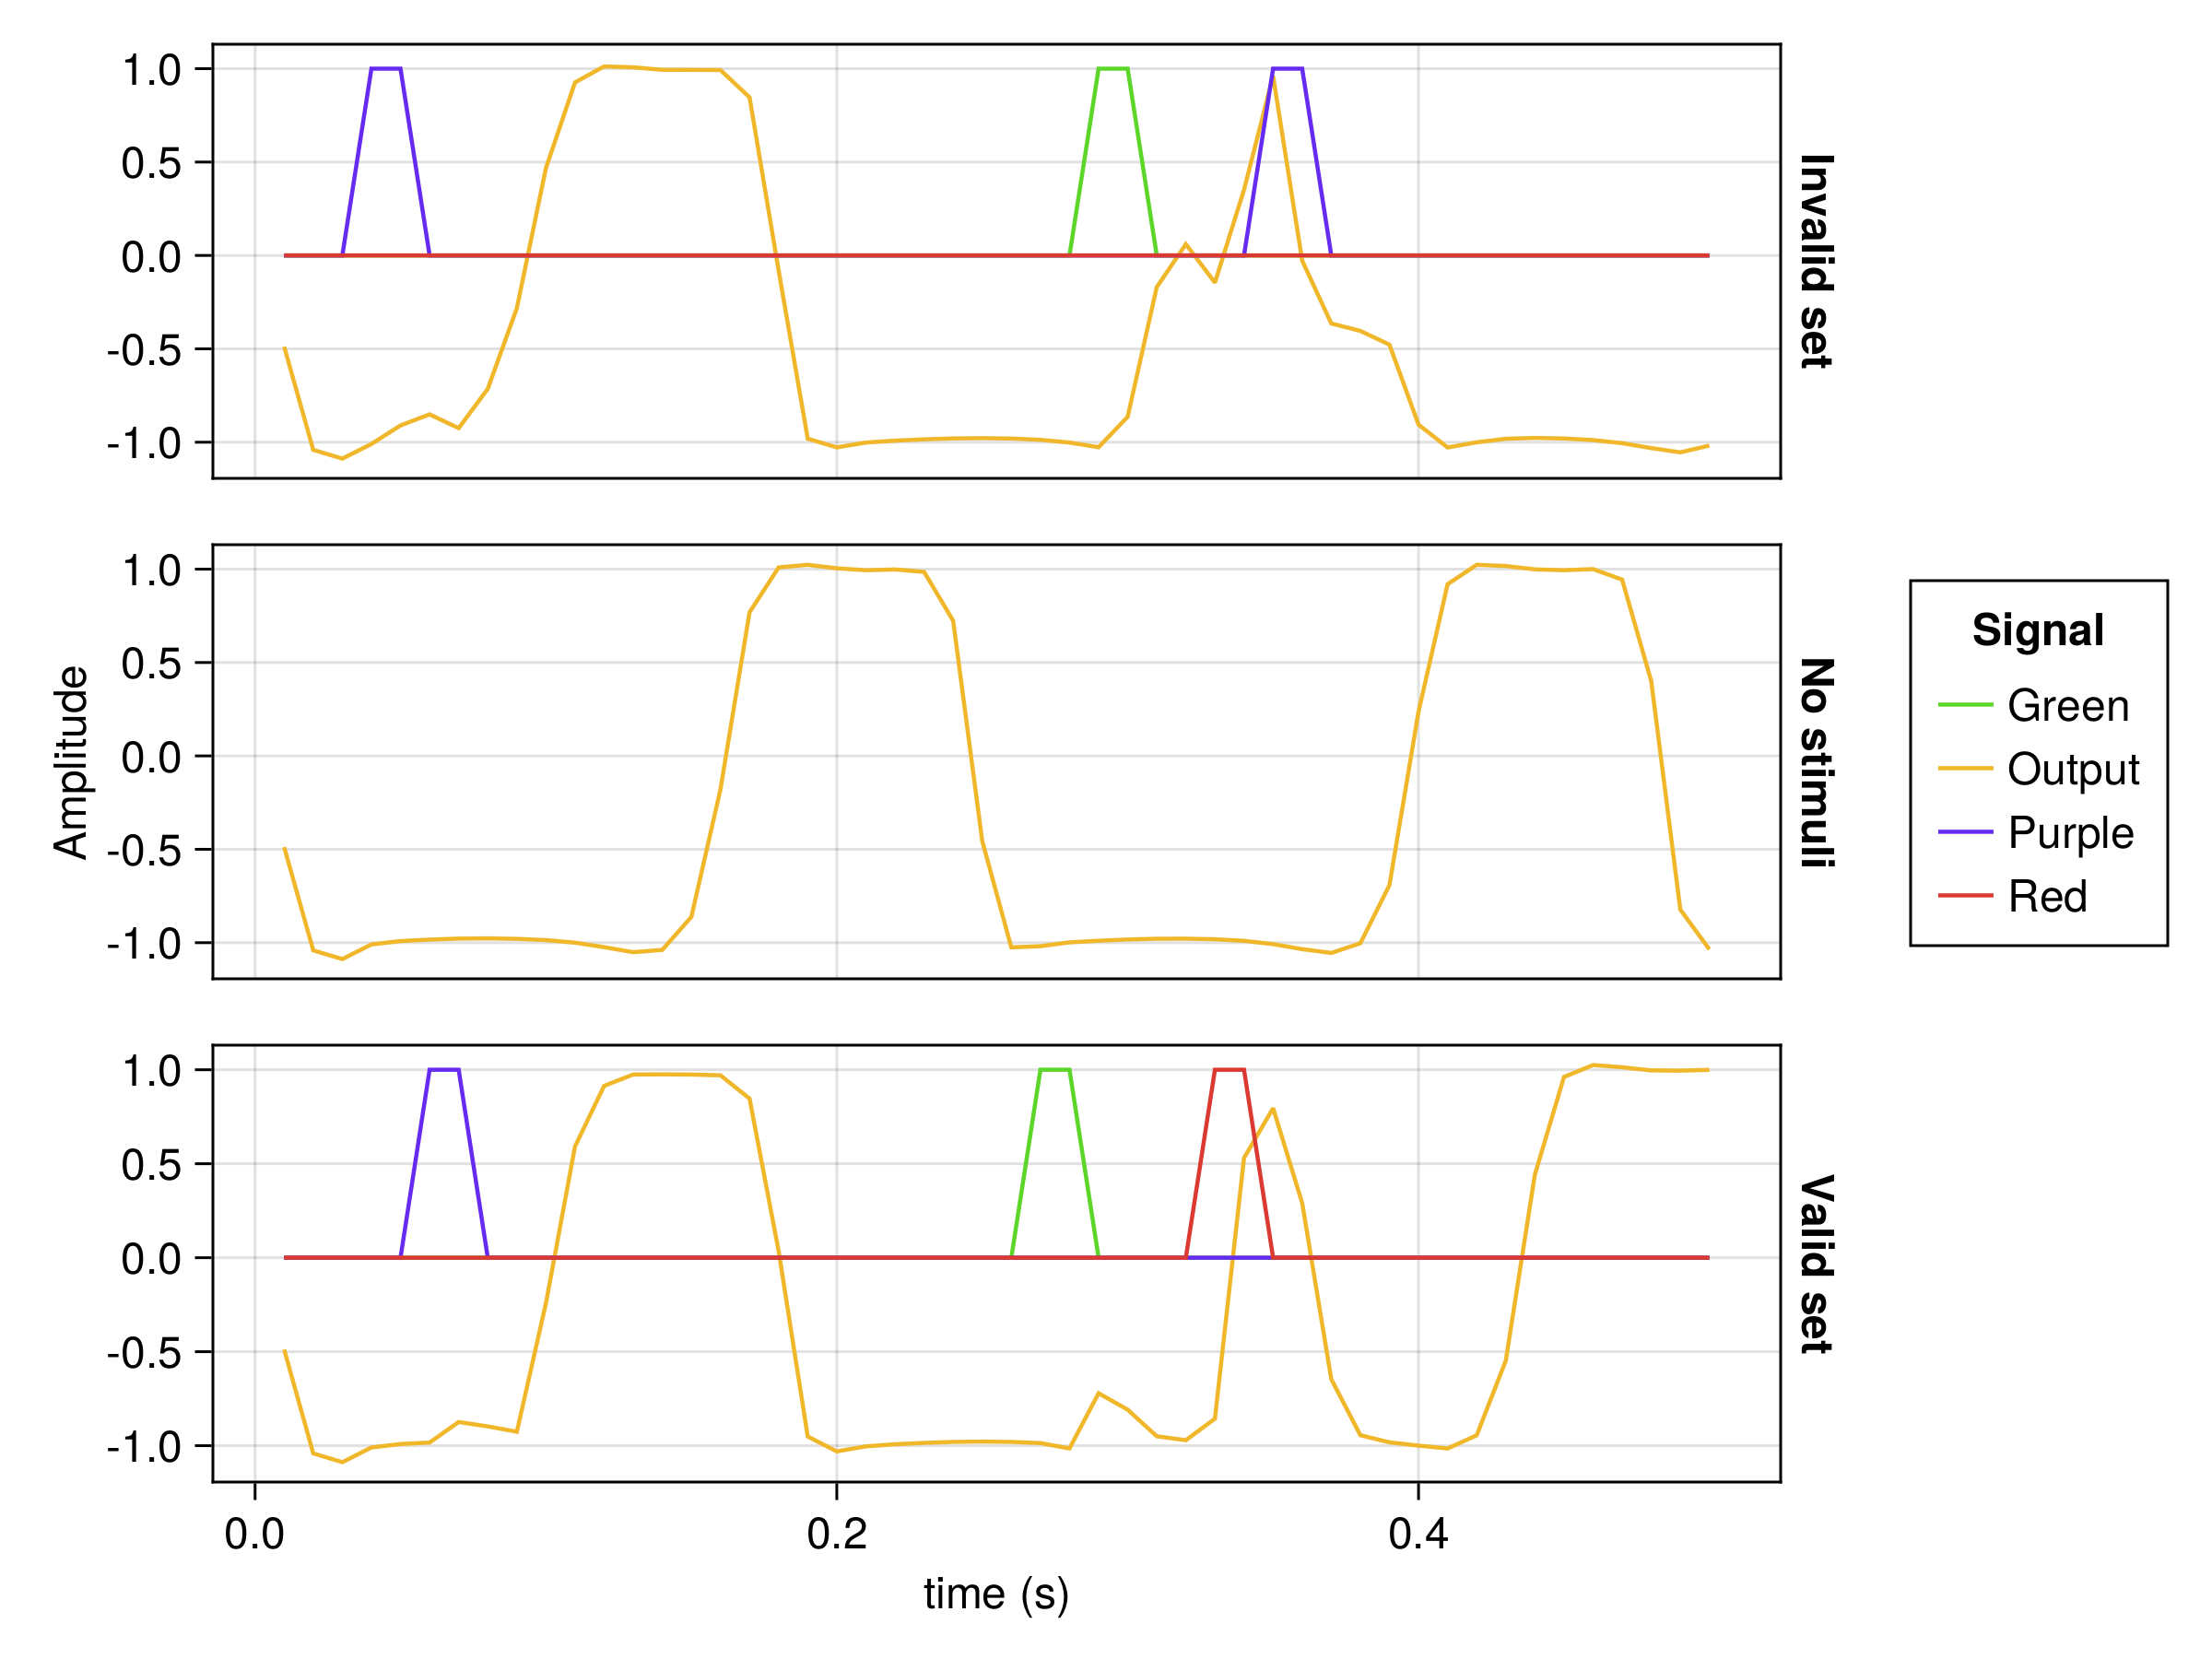
\includegraphics[scale=0.10]{SET_examples.png}}
\caption{Three examples of stimuli presented during trials and the models associated output. The top row shows a valid pattern trial, resulting in a model output of $+1$. The middle row presents a trial with no color stimulus and demonstrates the model completing two full oscillations in a single trial. The bottom row shows an invalid pattern trial, resulting in a model output of $-1$. Note the \textit{perturbations} due to stimulus presentation in the top and bottom rows.}
\label{exampletrialstimuli}
\end{figure}

For valid patterns, the model's output completes the trial in the positive phase of its underlying oscillation, generating a value of $+1$. Conversely, for invalid patterns, the output concludes the trial in the negative phase of its oscillation, yielding a value of $-1$. In the absence of a stimulus input, the model is observed to complete two oscillations within a single trial. The \textit{perturbations} corresponding to stimulus presentation indicate the influence of the stimulus on the oscillation, yet their computational significance remains unclear without further PCA analysis.

\subsection{PCA results}

The PCA of the model's firing rates revealed that the model had learned a low-dimensional limit cycle\footnote{Refer to \cite{strogatz2018nonlinear} for an overview of limit cycles in nonlinear dynamics.} that completed two full rotations during a trial (Fig.~\ref{pcasummary}). At the end of the trial, PCA reveals that the activations of the model would lie in one of three distinct locations along the limit cycle. Two locations represent invalid patterns while one location represents valid patterns. This dynamical behavior indicates that stimulus would shift the phase of the limit cycle in the model. This may be the computational affect of the \textit{perturbations}  seen in Fig.~\ref{exampletrialstimuli}.

\begin{figure}[htbp]
\centerline{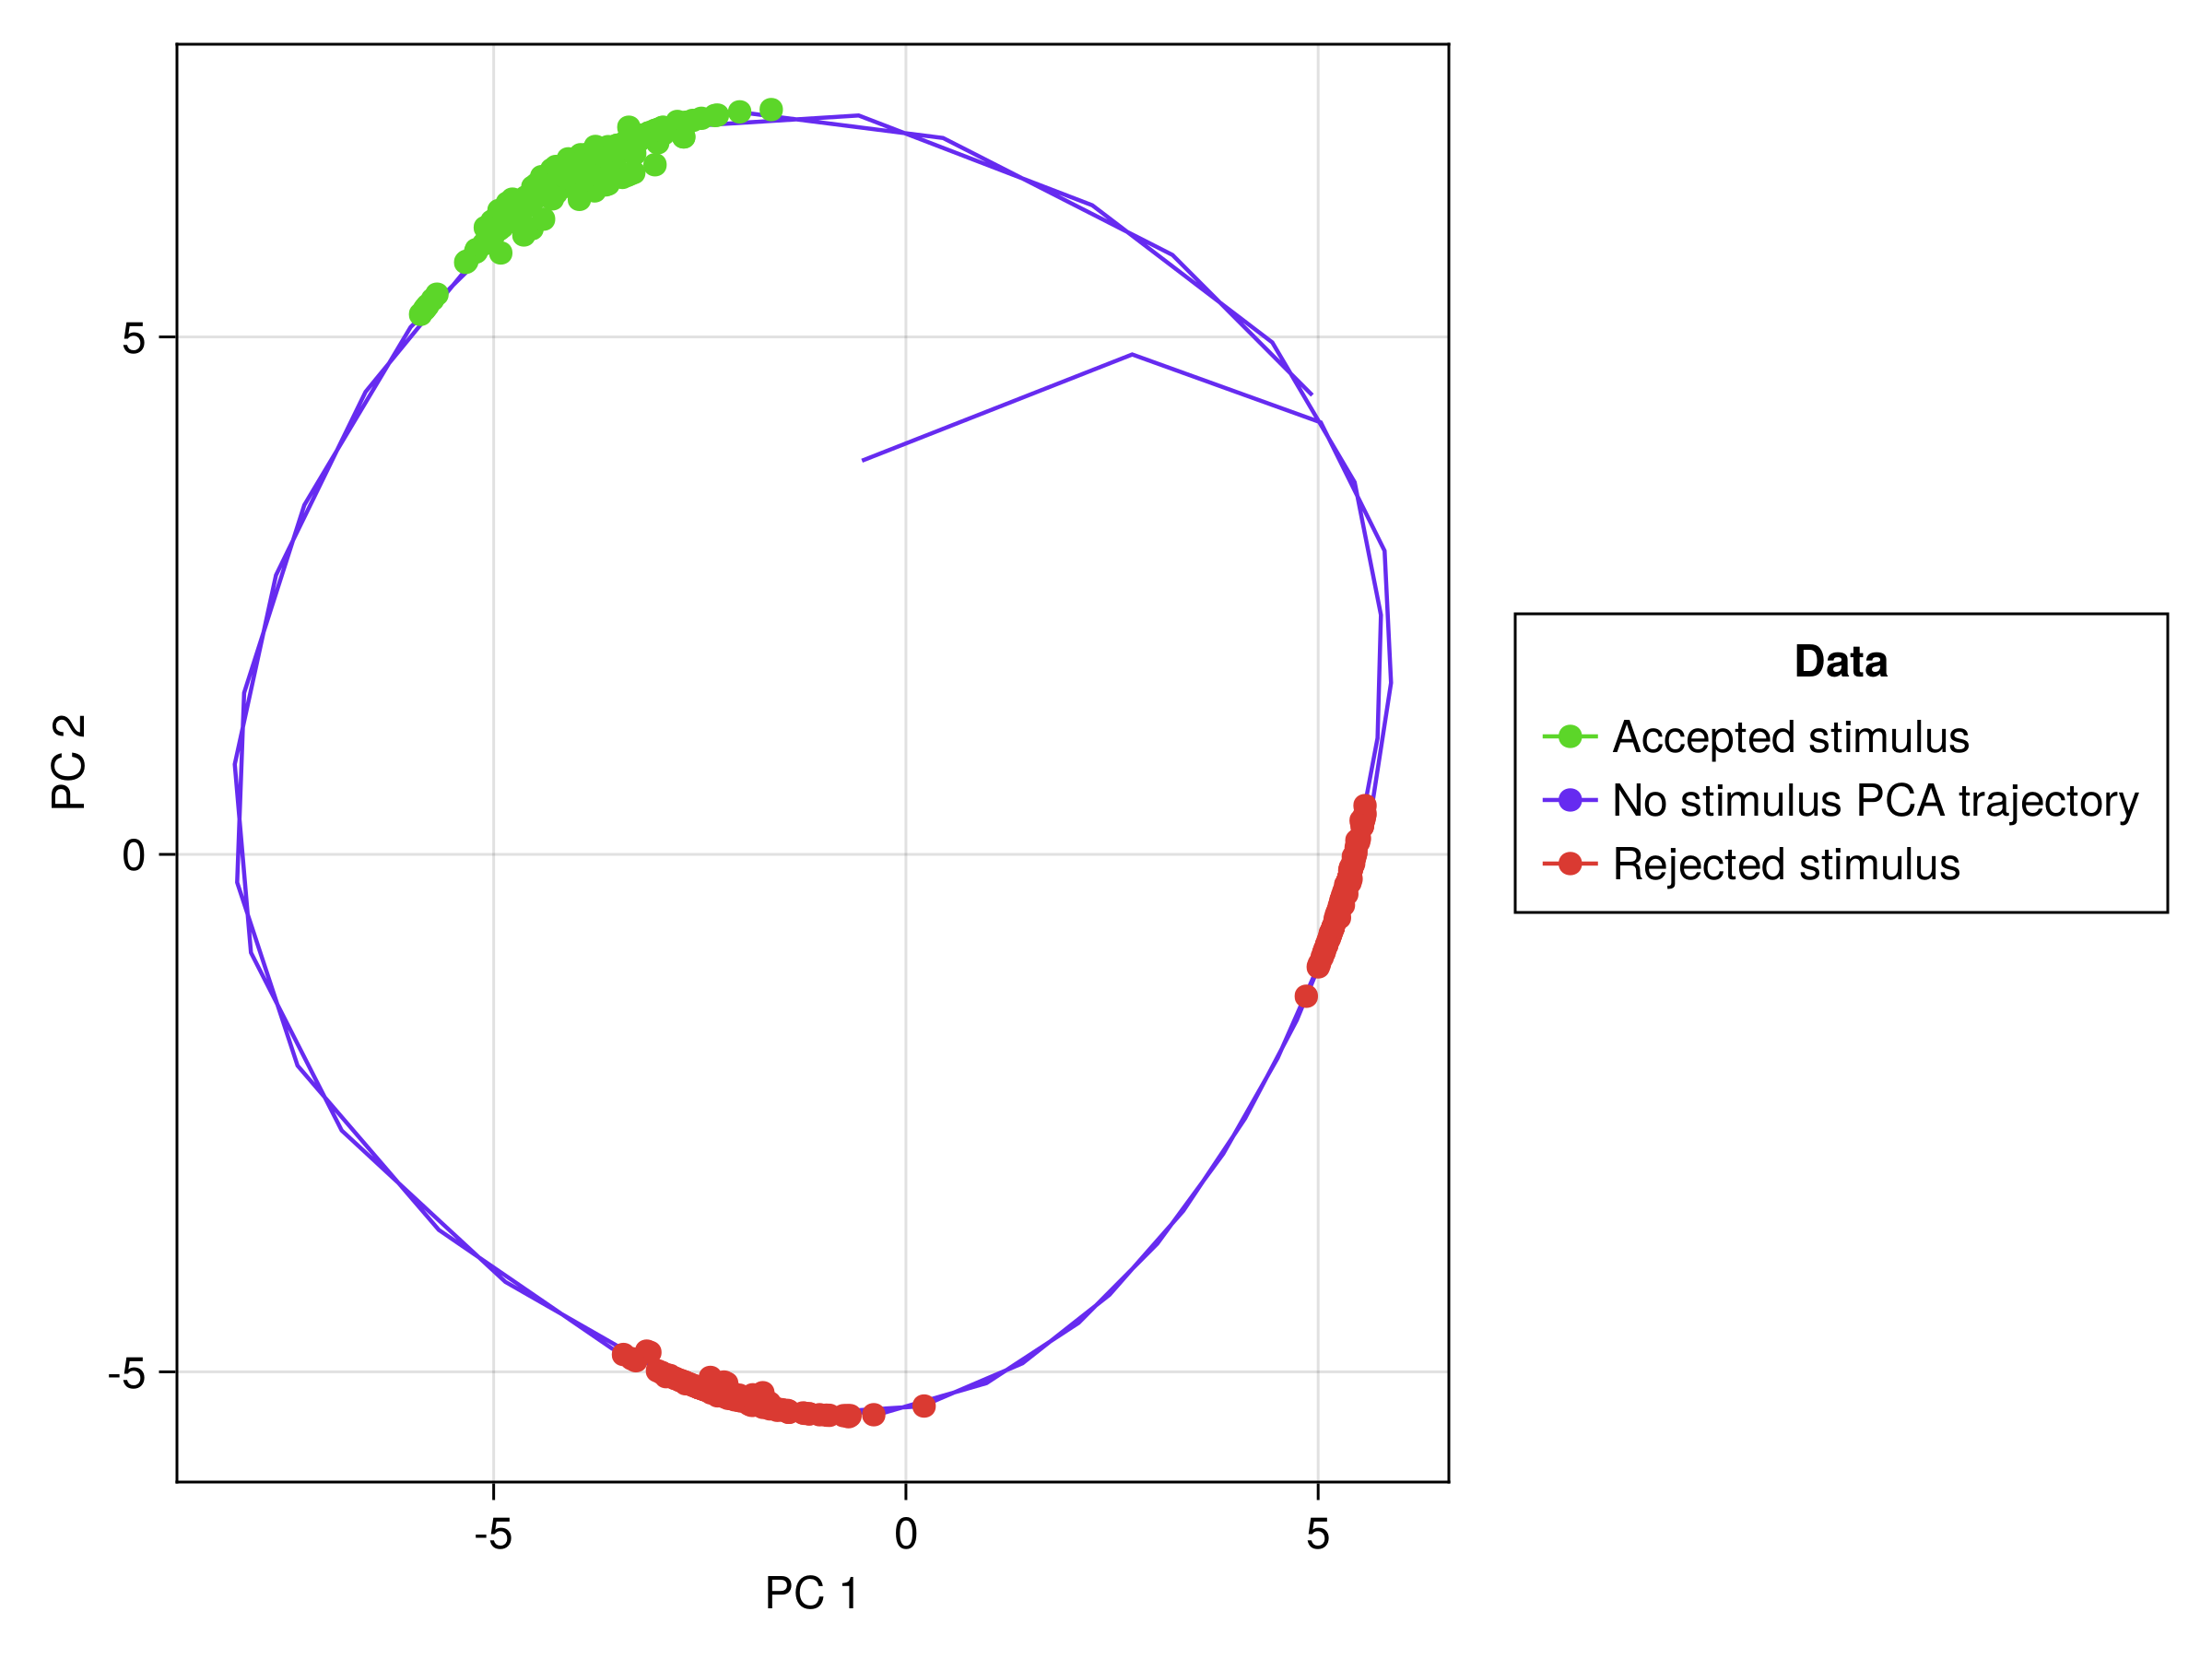
\includegraphics[scale=0.10]{pca_summary.png}}
\caption{This figure illustrates a low-dimensional representation of the model's trajectories, showing distinct clusterings at the endpoints of both accepted and rejected patterns. The trajectory validates the underlying dynamics of the model as a limit cycle. The clusterings at the endpoints of trajectories for accepted and rejected patterns imply that stimulus presentations induce phase shifts along this limit cycle.}
\label{pcasummary}
\end{figure}

To confirm that stimulus presentation resulted in phase-shifts along the limit cycle in the model, we further investigated the low-dimensional trajectories of the model by rotating the PCA data and visualizing the rotated PCA trajectories. Notice how in Fig.~\ref{pcasummary} if data were to be projected onto principal component (PC) 1, then the distribution of valid pattern PCA endpoints would mix with the distribution of invalid pattern PCA endpoints. By rotating PCA data by $60$ degrees, the distributions of valid and invalid pattern endpoints are linearly separable when projected onto PC 1.

Fig.~\ref{pcaacceptedsets} presents the dynamics of the model projected onto PC 1 over time for various trials. By comparing the impact of stimuli from different trials on the dynamics, we can formulate preliminary theories about how stimulus presentation influences the dynamics of the underlying limit cycle.  

\begin{figure}[htbp]
\centerline{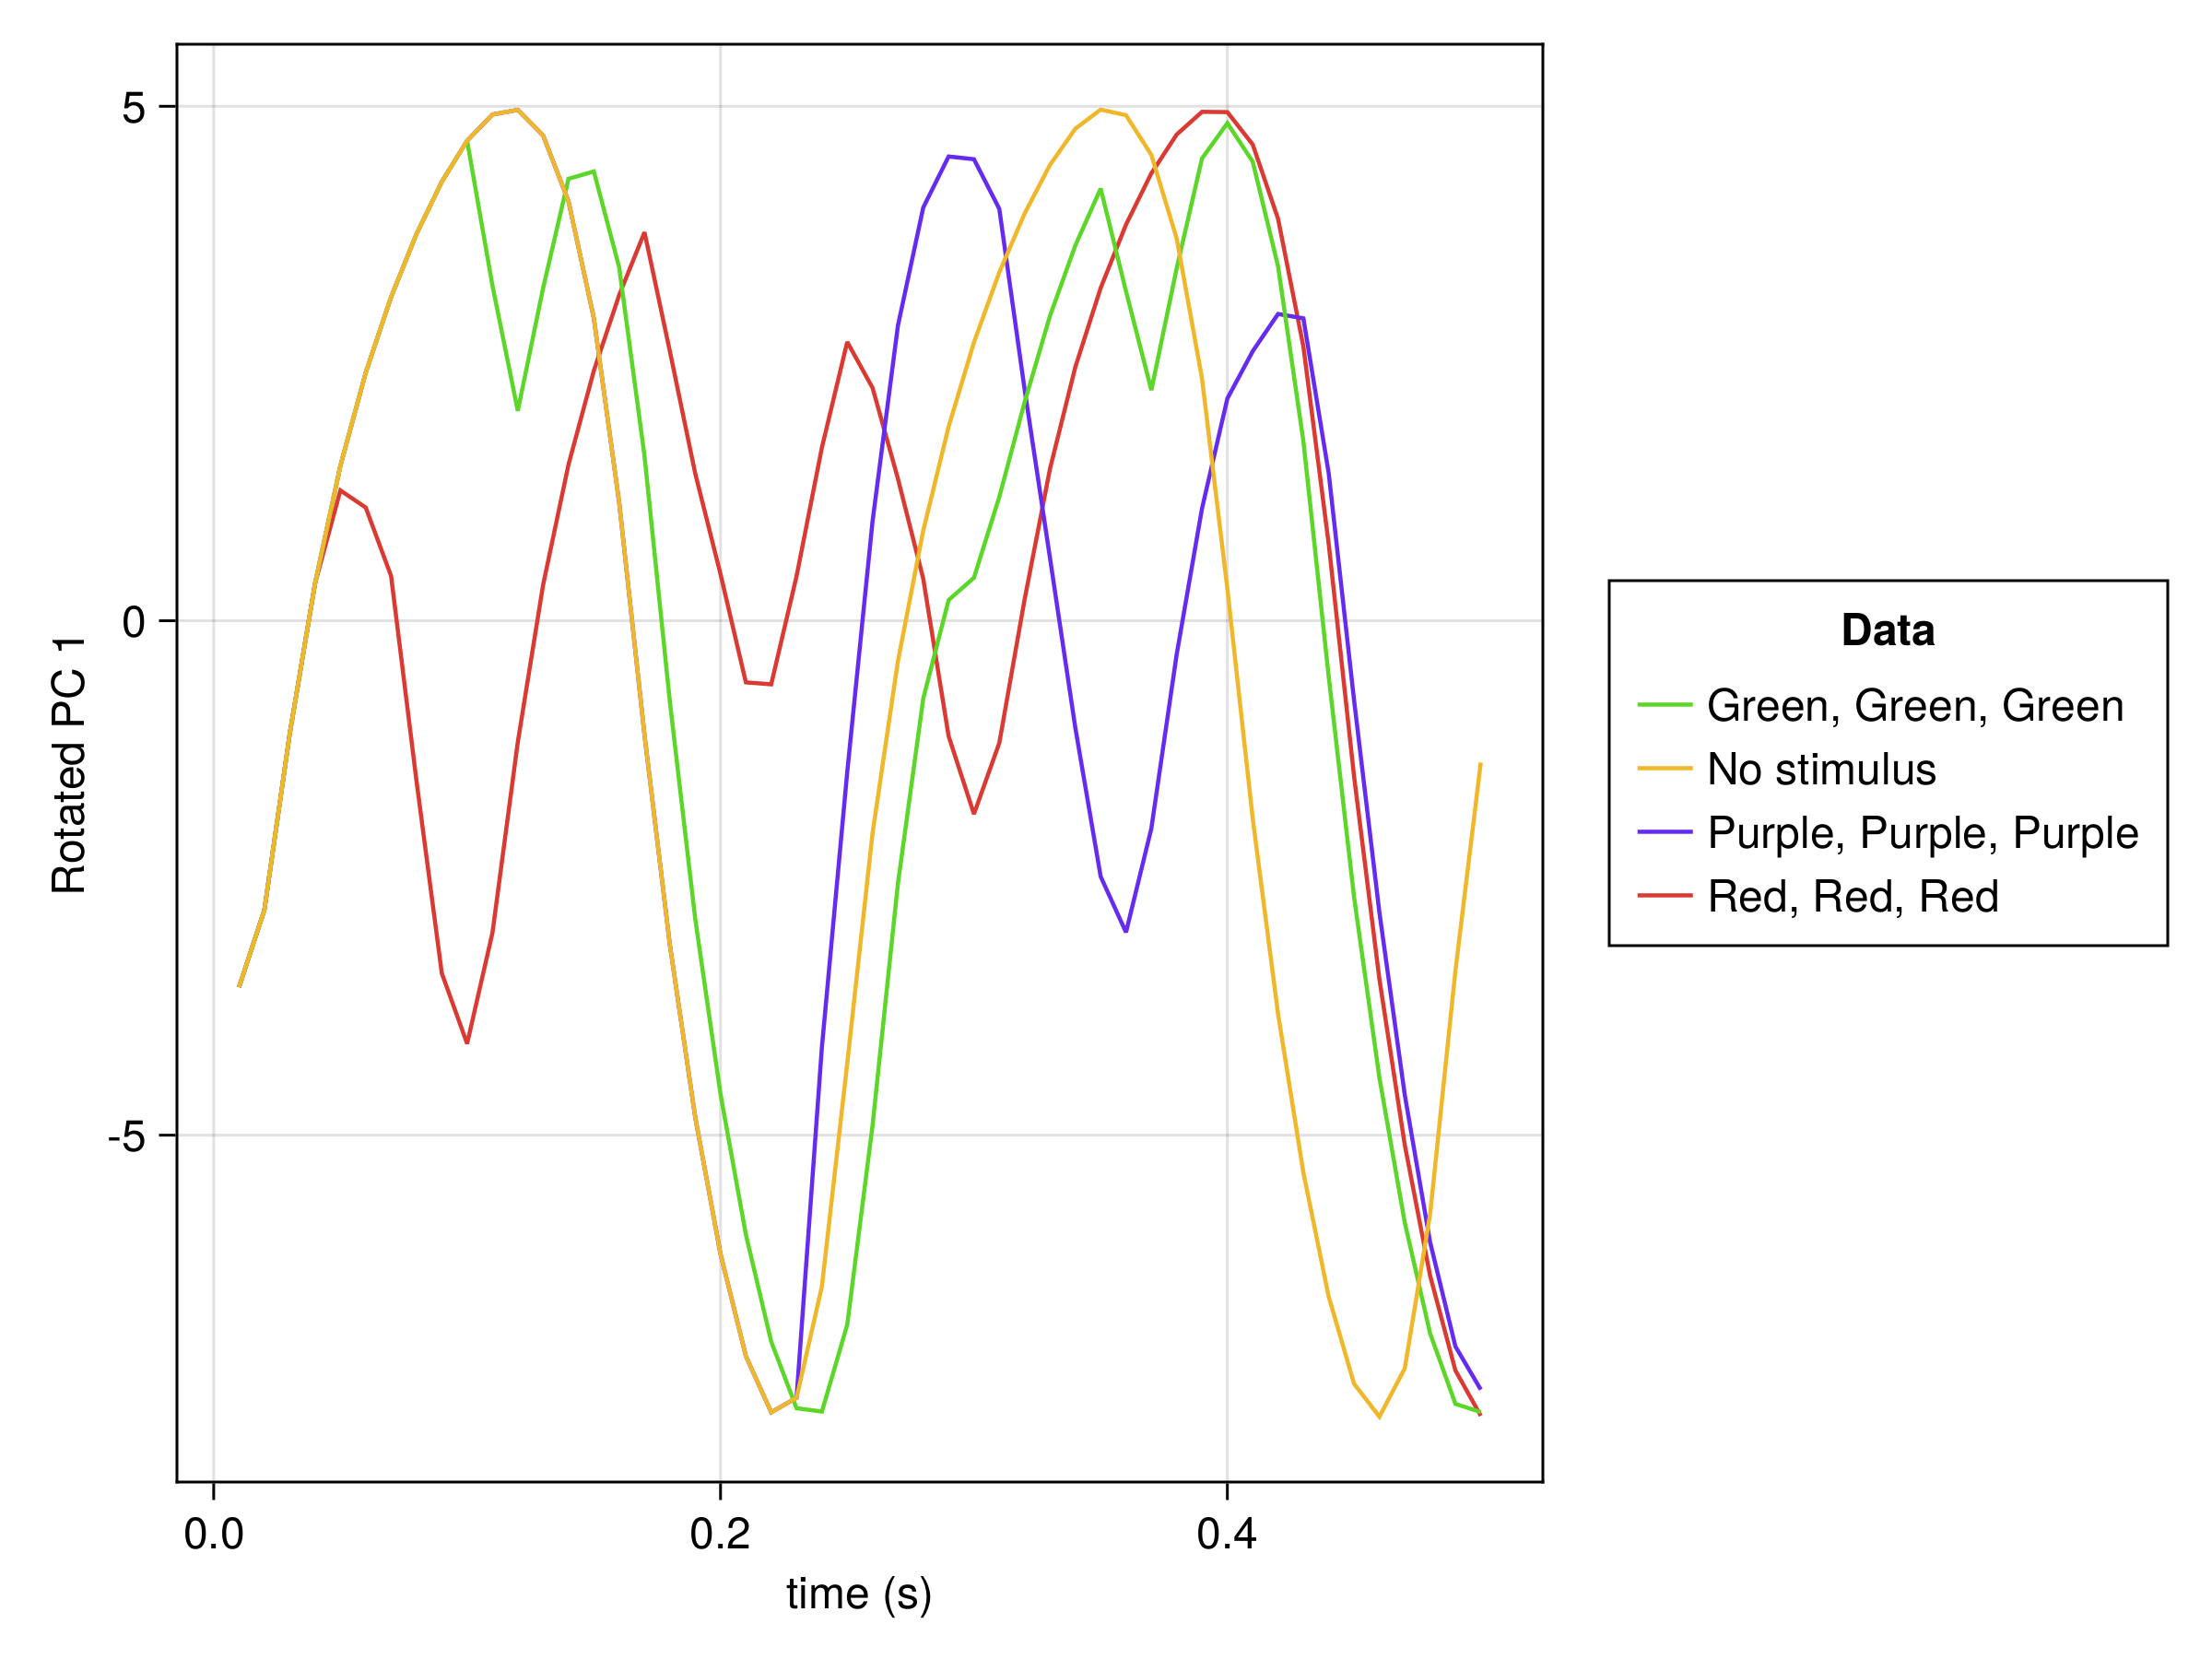
\includegraphics[scale=0.10]{rotated_pc1_accepted.png}}
\caption{This figure depicts the model's firing rates across four trials with various stimuli, projected onto the rotated PC 1 over time. The influence of stimulus presentation on the dynamics of the rotated PC 1 is visible. The Green, Green, Green trial shows minimal change compared to the no stimulus trial. When comparing the Red, Red, Red trial to the Purple, Purple, Purple trial, it appears that the red stimulus may reduce the phase of the oscillation while the purple stimulus may increase it.}
\label{pcaacceptedsets}
\end{figure}

A trial with all green stimuli appears to only slightly perturb the model's dynamics compared to a trial with no stimulus (Fig.~\ref{pcaacceptedsets}). Red stimuli seem to briefly \textit{reset} the network's dynamics, whereas purple stimuli cause the oscillation to \textit{jump} in phase. While these initial theories are somewhat broad, they offer a starting point for further investigation.

In light of the initial hypothesis positing a FSA with nodes representing fixed-points in the model, the theories developed from Fig.~\ref{pcaacceptedsets} prompt us to update our hypothesis. Given the presence of three distinct endpoint distributions (Fig.~\ref{pcasummary}) and phase-shifts marking transitions between these distributions, our updated FSA now includes three nodes. In this updated model, stimulus input induces transitions between nodes, and each node corresponds to a specific phase angle, instead of a fixed-point, within the model (Fig.~\ref{resultingfsa}). We have revised our initial assumption that all stimulus inputs of a particular color should point in the same direction. Instead, we now propose that all stimulus inputs must similarly affect the phase of the oscillation.

\begin{figure}[htbp]
\centerline{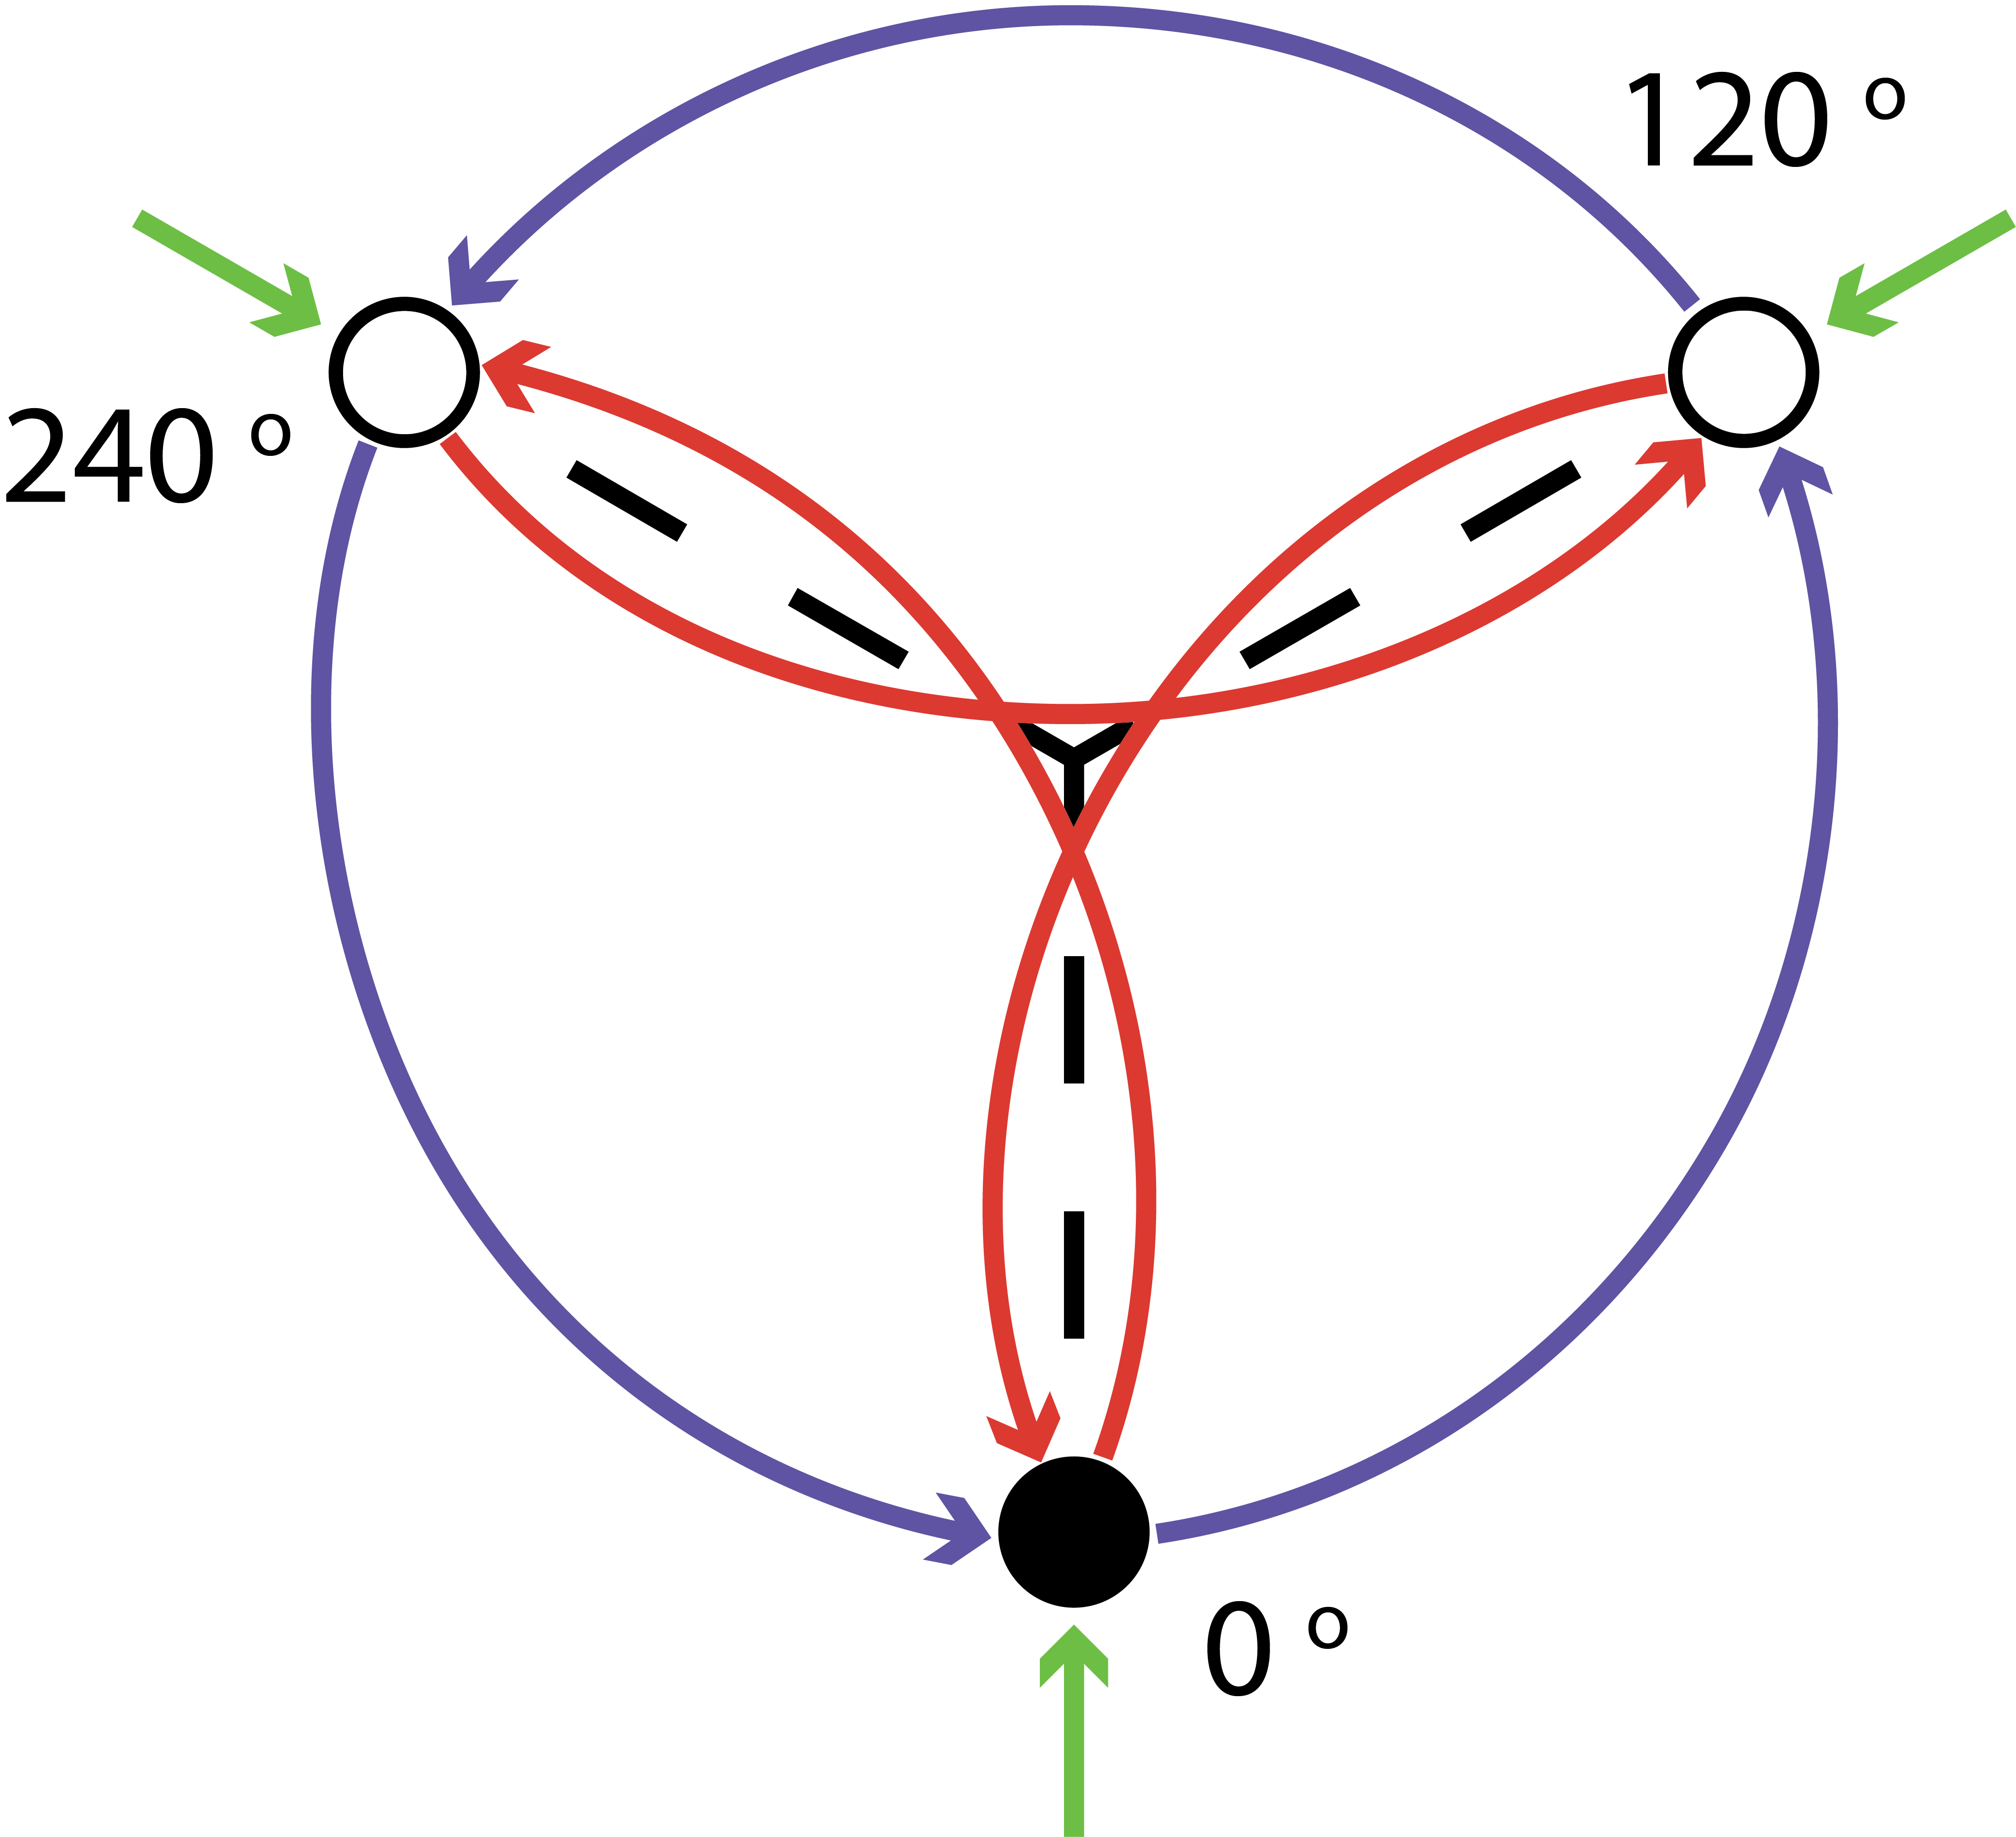
\includegraphics[scale=0.125]{resulting_FSA.png}}
\caption{This figure depicts the updated FSA that represents the underlying dynamics and computation of our trained model. The model begins at a phase angle of $0$ degrees, and stimulus presentations trigger transitions to other nodes, each representing a distinct phase angle.}
\label{resultingfsa}
\end{figure}

While we previously observed that green stimuli do impact the dynamics of the model (Fig.~\ref{exampletrialstimuli}), we simplify our model by assuming that green stimuli do not affect the underlying phase angle. Purple stimuli are postulated to add $120$ degrees to the phase angle, while red stimuli subtract $120$ degrees. If all stimuli are either \textit{uniform} or \textit{heterogeneous}, the phase angle shifts sum to $0$, causing the oscillation to land in an accepting phase.

To test the accuracy of this FSA model, we made predictions about the phase at which the model will conclude for invalid stimuli. For instance, if the stimulus pattern is purple, green, purple, then the model should end $120$ degrees behind the accepting patterns. If the stimuli is red, green, red, then the model should end $120$ degrees ahead of the accepting patterns. Fig.~\ref{pcarejectedsets} confirms these predictions and supports the validity of our new FSA model.

\begin{figure}[htbp]
\centerline{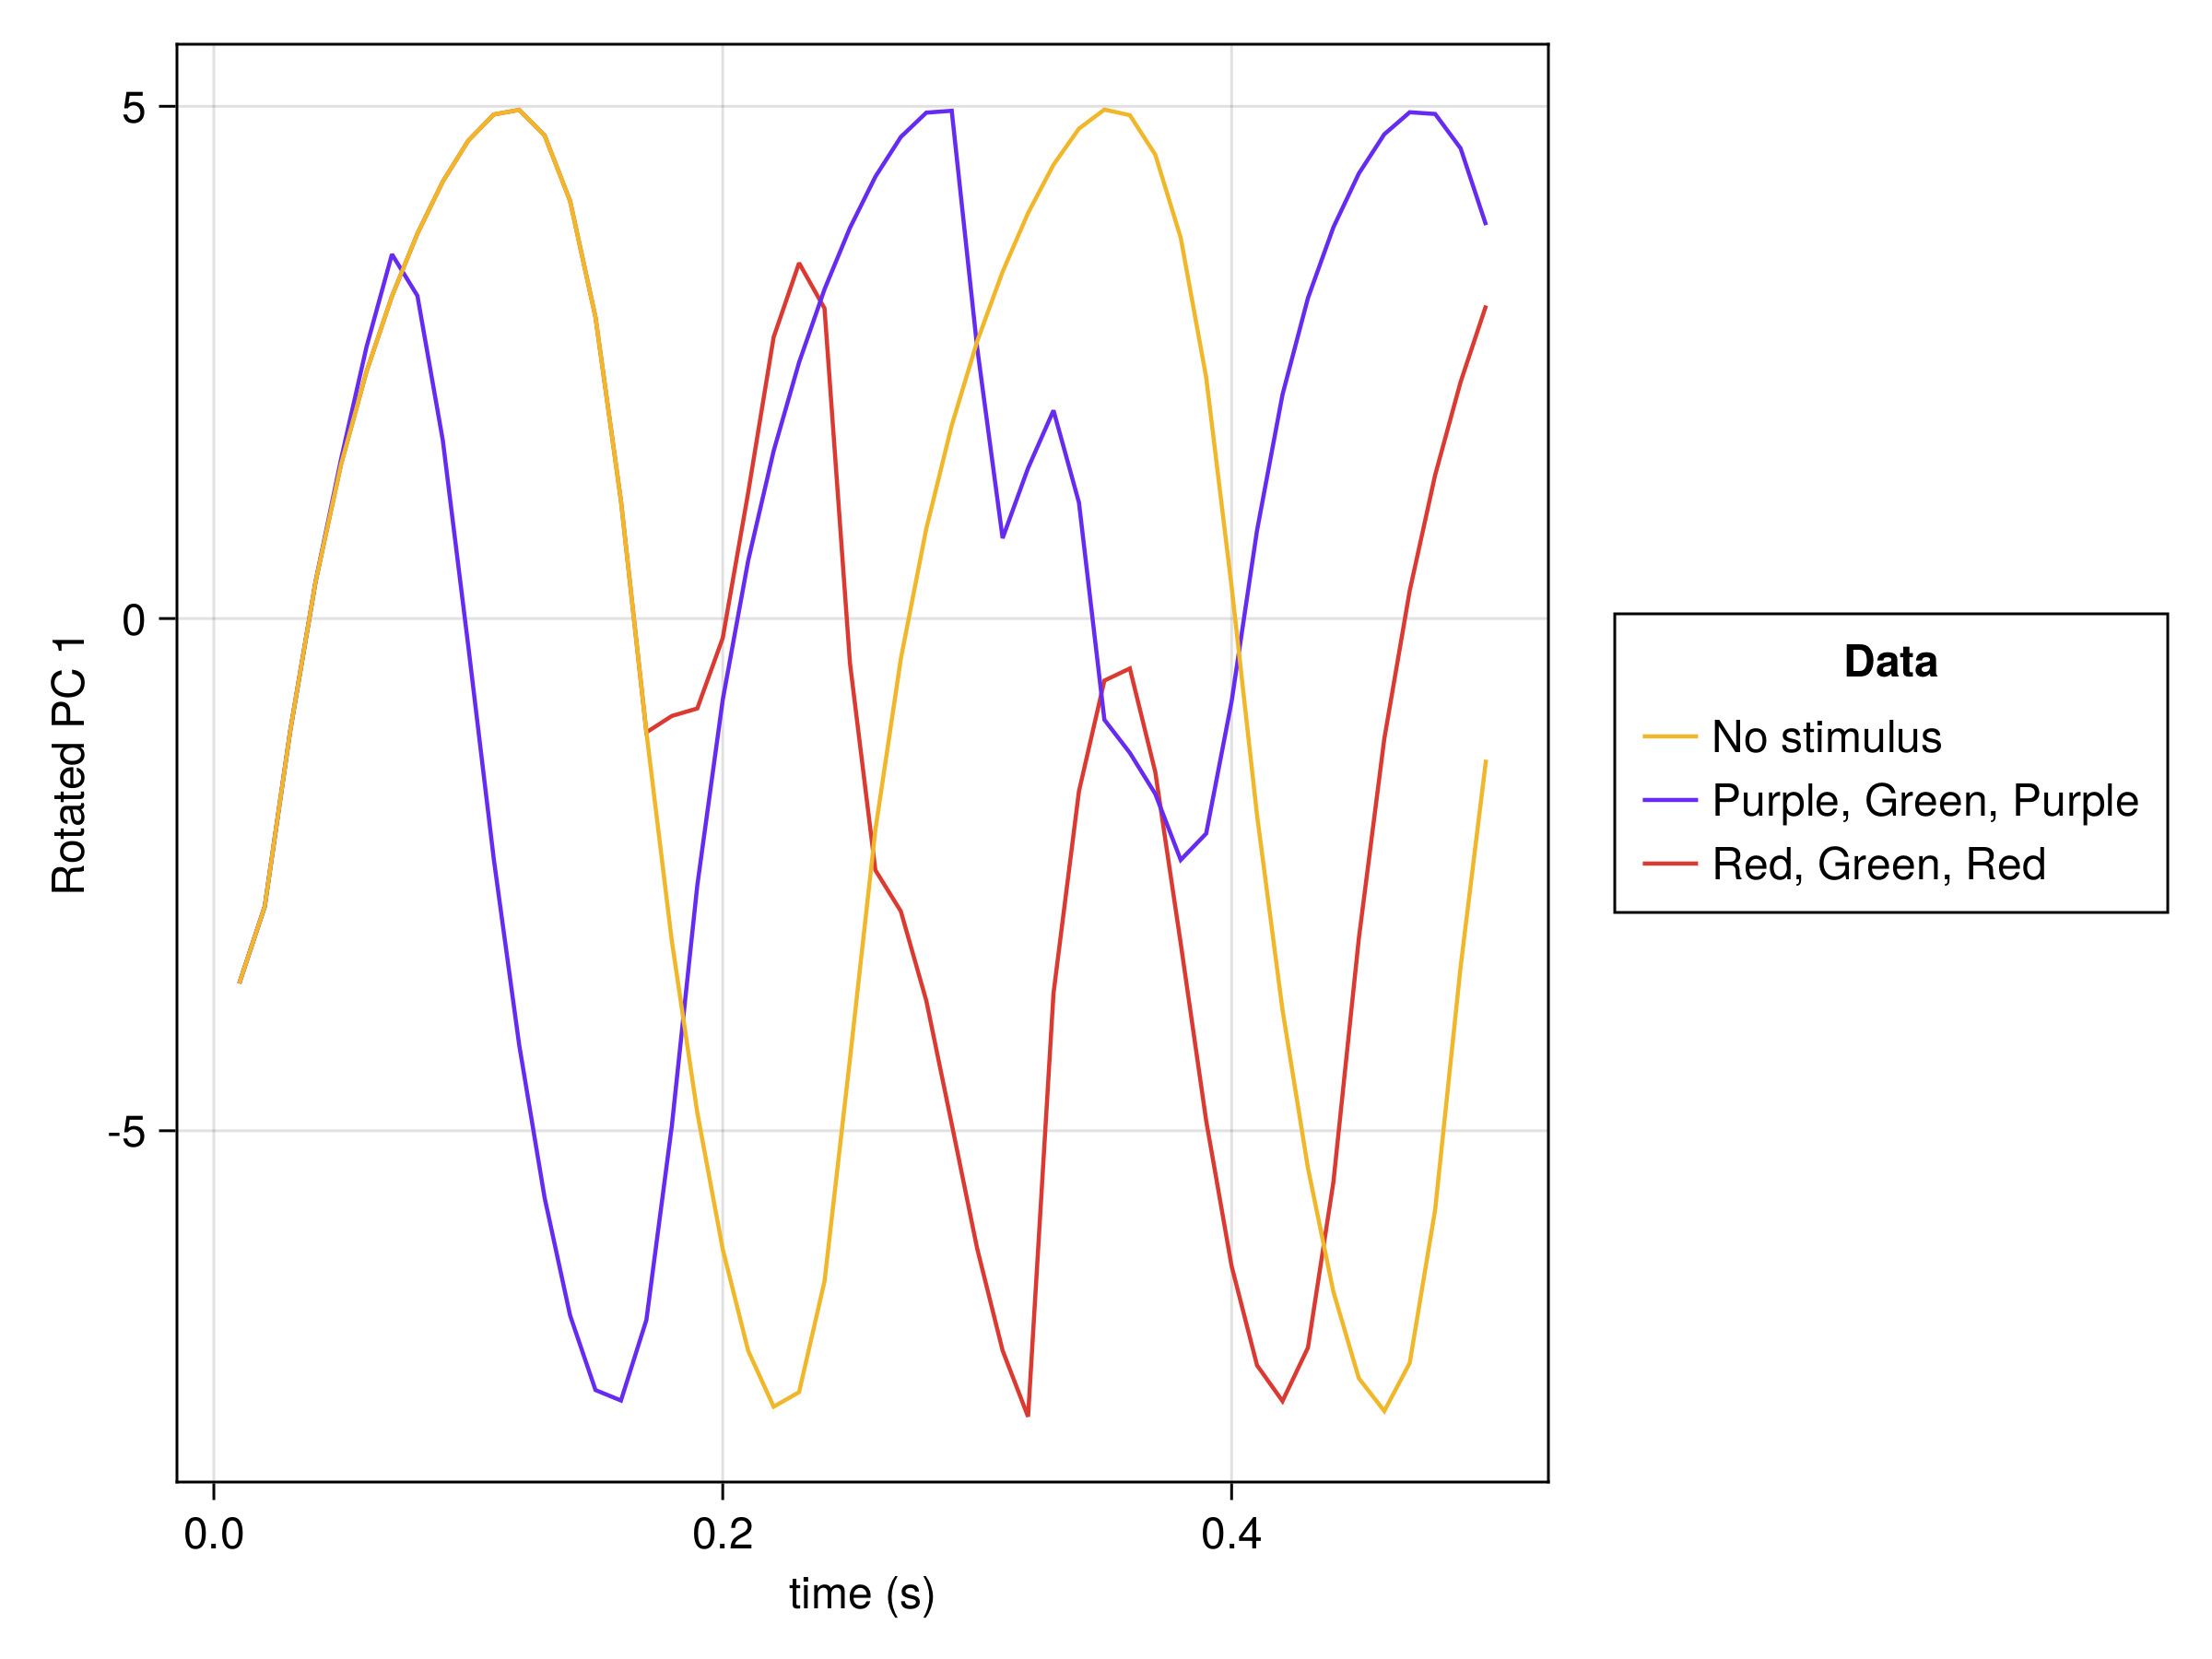
\includegraphics[scale=0.10]{rotated_pc1_rejected.png}}
\caption{This figure illustrates the projected trajectories of several invalid patterns onto the rotated PC 1. The depicted trajectories confirm the model's behavior according to our updated FSA, validating our predictions about the final phase for different stimulus sequences.}
\label{pcarejectedsets}
\end{figure}

\subsection{Simplifying the model}

To deepen our understanding of the underlying computations in our model, we developed a new, simpler model that could replicate the dynamics of the original one. This process would further validate the FSA representation of our model's pattern recognition capabilities (Fig.~\ref{resultingfsa}). The dynamics of the rotated PC 1 of our model can be expressed with the following equation:

\begin{equation}
f(t) = 7\sin (\frac{2\pi}{0.29}t+\sum^t_{t_o=1}\phi(t_o))-1.5\label{simpmodel}
\end{equation}

In (\ref{simpmodel}), $\phi(t)$ represents the pattern signal, which is $\frac{2\pi}{3}$ if the stimulus is purple, $-\frac{2\pi}{3}$ if the stimulus is red, and $0$ if the stimulus is green or if no stimulus is present.

It is important to note that (\ref{simpmodel}) simplifies many of the dynamical properties observed in the dynamics of rotated PC 1. We simplify the frequency of (\ref{simpmodel}) to be constant while it is evident that the rate of the dynamics around the limit cycle is nonuniform (Fig.~\ref{pcasummary}). In addition, the presentation of stimulus causes a dynamical response in the dynamics of the full model (Fig.~\ref{pcaacceptedsets}) and (\ref{simpmodel}) models these responses as being sharp transitions in phase. Yet, with these simplifications, we believe that (\ref{simpmodel}) captures the underlying computational mechanisms identified in the rotated PC 1.

As expected, this simplified model can accurately classify all trials, assuming there is no recurrent noise. Fig.~\ref{constructedmodel} displays a few examples of the dynamics of (\ref{simpmodel}) plotted alongside the actual dynamics of the Rotated PC 1 of the full model. The similarity between the trajectories of these two models provides additional validation for our FSA representation of the computations performed by our full model.

\begin{figure}[htbp]
\centerline{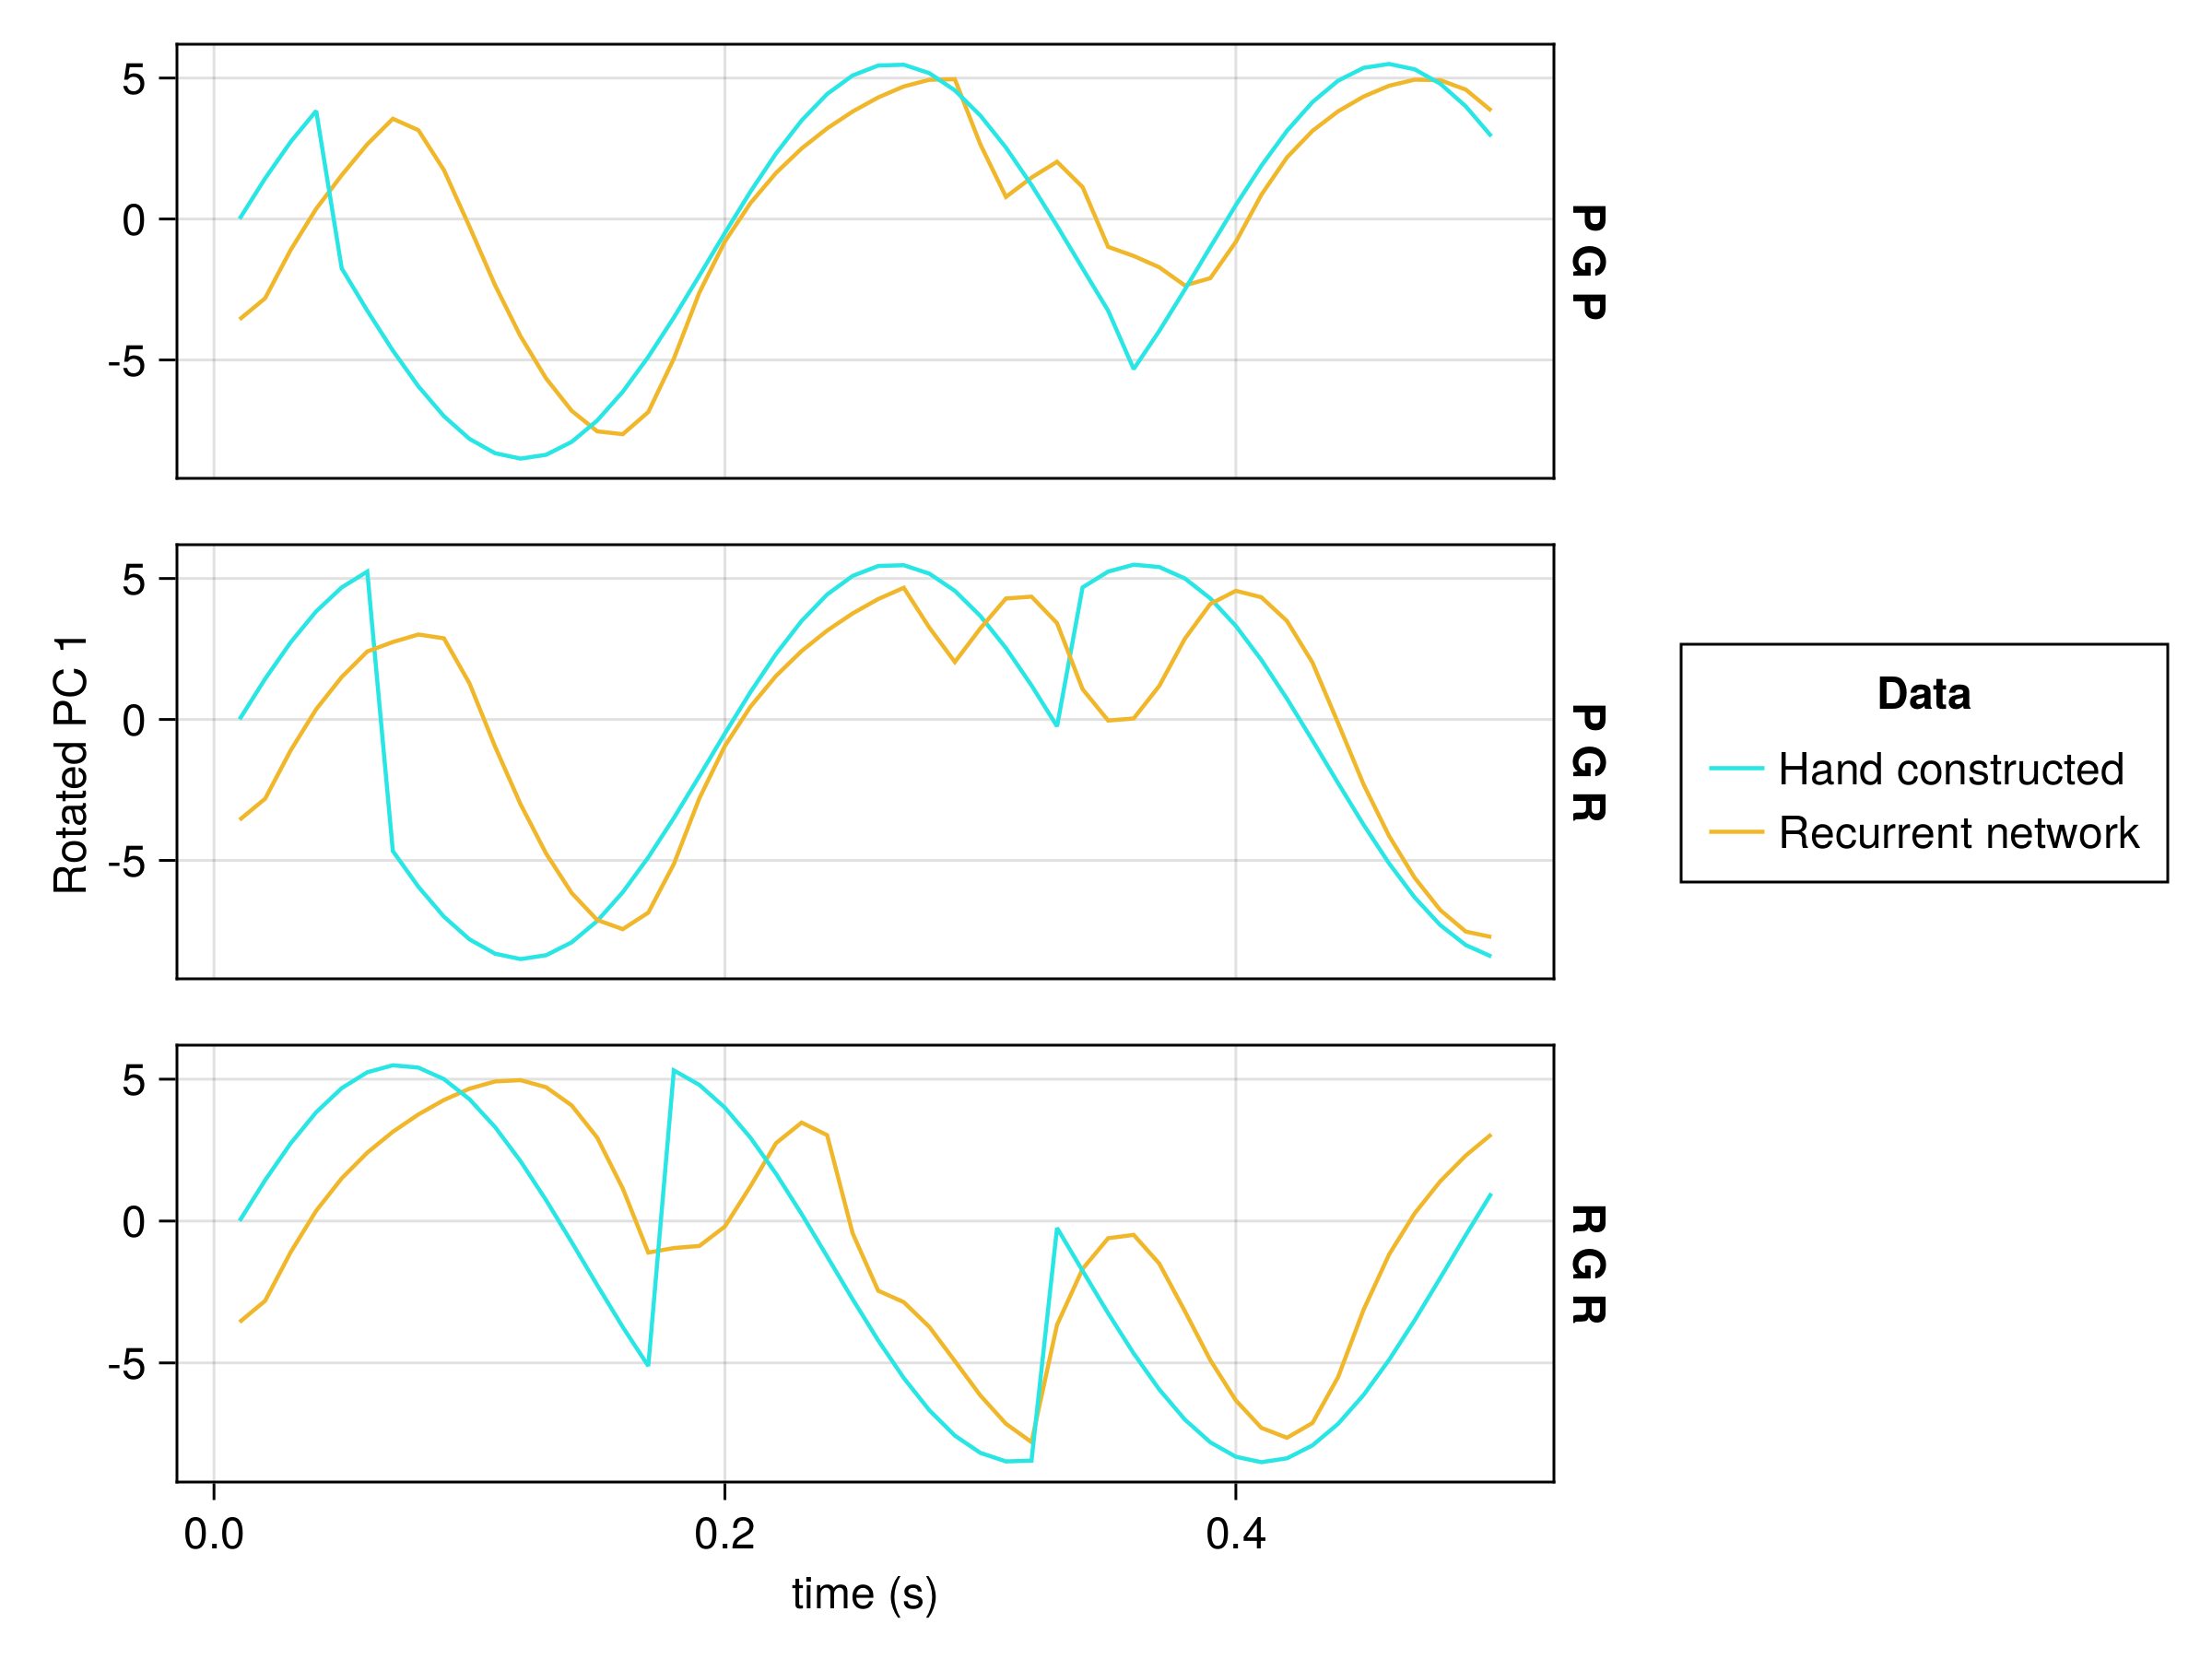
\includegraphics[scale=0.10]{constructed_phase_angle_computation.png}}
\caption{This figure illustrates three examples of the trajectories of our simplified model in comparison to the rotated PC 1 of the full model. The top row displays both models in a purple, green, purple trial. The middle row shows both models in a purple, green, red trial. The bottom row represents both models in a red, green, red trial.}
\label{constructedmodel}
\end{figure}

\section{Discussion}

In this study, we reveal a key mechanism through which an RNN, trained for pattern recognition in a task inspired by the SET card game, accurately recognizes all patterns devoid of noise. By interpreting pattern recognition through phase angle shifts in a low-dimensional limit cycle as transitions within a finite state automaton (FSA), we present a fresh perspective on the neural computations that underpin pattern recognition (Fig.~\ref{resultingfsa}). Notably, this finding underscores the ability to interpret the mechanisms learned by an RNN, a theme we will elaborate on throughout this discussion.

While there is a lengthy precedent of FSAs being employed to model human cognition \cite{b26}, our knowledge has yet to widely extend to the neural circuit-level implementation of these FSAs. Our study fills this gap, presenting an FSA learned within an RNN, a biologically plausible model. Nevertheless, we caution that this finding primarily pertains to a single attribute and simple \textit{uniform} or \textit{heterogeneous} patterns, necessitating further investigation to ascertain its applicability to more complex pattern recognition problems.

This work's significance lies in contributing to an expanding understanding of the neural computations underpinning pattern recognition, paving the way toward a more comprehensive grasp of neural computation. Echoing the findings from \cite{mante2013context}, the dynamical mechanisms unveiled in this study could likely be found in the prefrontal cortex of primates executing similar pattern recognition tasks. While prior studies provided evidence of accumulation and decision-making \cite{chaisangmongkon2017computing}, the complexity of stimuli was relatively simple. Only biological evidence can determine whether the neural dynamics underlying pattern recognition are oscillatory or attractive.

We ambitiously look forward to extending this work by exploring the integration of oscillators with other dynamical motifs to model higher-order cognitive behaviors \cite{driscoll2022flexible}. This parallels the compilation of logical operations into algorithms and computer programs, underscoring the analogies between biological and artificial computational systems \cite{jaeger2021towards}.

Furthermore, in the context of neural circuit-level FSA implementations, we note our work's novelty. Previously, it was postulated that a Hopfield network could be represented as the average phase in a system of weakly coupled oscillators \cite{hoppensteadt1999oscillatory}. Existing work also demonstrated RNNs' ability to retain stimuli in the phase shift of a coupled oscillator system \cite{pals2023trained}. We build on these studies to show that RNNs can implement sequential pattern recognition in limit cycles like FSAs, potentially hinting at computational mechanisms for brain oscillations.

Contrasting with other computational neuroscience work proposing oscillatory computational mechanisms, which often presumes neurons to oscillate \cite{hoppensteadt1999oscillatory}. or receive oscillatory input \cite{pals2023trained}, our model makes no such assumptions and learns an oscillatory mechanism. However, our work's limitations should be acknowledged: PCA only uncovers correlations without revealing causal mechanisms \cite{langdon2022latent}, and the recognized patterns are rule-based and simple.

The emergence of limit cycles rather than attractor networks, owing to the compact realization of FSAs, raises a fascinating question. The observed oscillatory activity may be attributed to task-specific implementations. Given that RNNs are universal function approximators \cite{b28}, there could be some parameters of our task that realize our initial hypothesis in a trained RNN (Fig.~\ref{hypothesisFSA}).

Future investigations could focus on developing a more descriptive simplified model of the RNN that incorporates the dynamics of phase shifts induced by stimuli, instead of instantaneous shifts (Fig.~\ref{constructedmodel}). They could also explore how these FSA models of pattern validation integrate into visual search for comprehensive SET playing, and the potential application of cognitive technologies using oscillations for cognitive-like computations.

Our work not only offers new insights into the neural computations underpinning pattern recognition but also illuminates the interpretability of mechanisms learned by RNNs. In a field where interpretability is becoming increasingly valuable, this serves as a clear and important example of how these mechanisms can be easily understood and interpreted. This will undoubtedly be of interest to the machine learning community, which is making concerted efforts to understand the mechanisms in deep learning models \cite{nanda2023progress}. In sum, this study presents a significant stride toward a more comprehensive understanding of neural computations and their implementation in pattern recognition tasks.

\section*{Acknowledgment}

We would like to thank Nikasha Patel, Brabeeba Wang, Sabrina Drammis, and Nancy Lynch for helpful discussions pertaining to the conceptualization of this work. We would also like to acknowledge the assistance of OpenAI's ChatGPT in editing portions of the manuscript.

\begin{thebibliography}{00}
\bibitem{inhelder1964early} B. Inhelder and J. Piaget, ``The Early Growth of Logic in the Child: Classification and Seriation,'' Routledge, 1964.
\bibitem{bishop2006pattern} C. M. Bishop and N. M. Nasrabadi, ``Pattern recognition and machine learning,'' Springer, 2006.
\bibitem{lecun2015deep} Y. LeCun, Y. Bengio, and G. Hinton, ``Deep learning,'' Nature, 2015.
\bibitem{sussillo2013opening} D. Sussillo and O. Barak, ``Opening the black box: low-dimensional dynamics in high-dimensional recurrent neural networks,'' Neural Computation, vol. 25, no. 3, pp. 626--649, 2013.
\bibitem{mante2013context} V. Mante, D. Sussillo, K. V. Shenoy, and W. T. Newsome, ``Context-dependent computation by recurrent dynamics in prefrontal cortex,'' Nature, vol. 503, no. 7474, pp. 78--84, 2013.
\bibitem{driscoll2022flexible} L. Driscoll, K. Shenoy, and D. Sussillo, ``Flexible multitask computation in recurrent networks utilizes shared dynamical motifs,'' bioRxiv, 2022.
\bibitem{kay2022neural} K. Kay, X. Wei, R. Khajeh, M. Beiran, C. J. Cueva, G. Jensen, V. P. Ferrera, and L. F. Abbott, ``Neural dynamics and geometry for transitive inference,'' bioRxiv, 2022.
\bibitem{pals2023trained} M. Pals, J. H. Macke, and O. Barak, ``Trained recurrent neural networks develop phase-locked limit cycles in a working memory task,'' bioRxiv, 2023.
\bibitem{sussillo2015neural} D. Sussillo, M. M. Churchland, M. T. Kaufman, and K. V. Shenoy, ``A neural network that finds a naturalistic solution for the production of muscle activity," Nature Neuroscience, vol. 18, no. 7, pp. 1025--1033, 2015.
\bibitem{cueva2018emergence} C. J. Cueva and X.-X. Wei, ``Emergence of grid-like representations by training recurrent neural networks to perform spatial localization," arXiv preprint arXiv:1803.07770, 2018.
\bibitem{strogatz2018nonlinear} S. H. Strogatz, ``Nonlinear Dynamics and Chaos: With Applications to Physics, Biology, Chemistry, And Engineering,'' CRC Press, 2000.
\bibitem{gordon2017joy} L. McMahon, G. Gordon, H. Gordon, and R. Gordon, ``The Joy of SET: The Many Mathematical Dimensions of a Seemingly Simple Card Game,'' Princeton University Press, 2017.
\bibitem{richards2019deep} B. A. Richards, T. P. Lillicrap, P. Beaudoin, Y. Bengio, R. Bogacz, A. Christensen, C. Clopath, R. P. Costa, A. de Berker, S. Ganguli, et al., ``A deep learning framework for neuroscience,'' Nature Neuroscience, vol. 22, no. 11, pp. 1761--1770, 2019.
\bibitem{bezanson2017julia} J. Bezanson, A. Edelman, S. Karpinski, and V. B. Shah, ``Julia: A fresh approach to numerical computing,'' SIAM Review, vol. 59, no. 1, pp. 65--98, 2017.
\bibitem{pal2022lux} A. Pal, ``Lux: Explicit Parameterization of Deep Neural Networks in Julia,'' GitHub repository, 2022, [Online]. Available: https://github.com/avik-pal/Lux.jl/.
\bibitem{rackauckas2020universal} C. Rackauckas, Y. Ma, J. Martensen, C. Warner, K. Zubov, R. Supekar, D. Skinner, A. Ramadhan, and A. Edelman, ``Universal differential equations for scientific machine learning,'' arXiv preprint arXiv:2001.04385, 2020.
\bibitem{rackauckas2017differentialequations} C. Rackauckas and Q. Nie, ``Differentialequations. jl--a performant and feature-rich ecosystem for solving differential equations in julia,'' Journal of Open Research Software, vol. 5, no. 1, 2017.
\bibitem{loshchilov2017decoupled} I. Loshchilov and F. Hutter, ``Decoupled weight decay regularization,'' arXiv preprint arXiv:1711.05101, 2017.
\bibitem{langdon2022latent} C. Langdon and T. A. Engel, ``Latent circuit inference from heterogeneous neural responses during cognitive tasks,'' bioRxiv, 2022.
\bibitem{b27} J. J. Hopfield, ``Neural networks and physical systems with emergent collective computational abilities,'' Proc. Natl. Acad. Sci., vol. 79, no. 8, pp. 2554--2558, 1982.
\bibitem{chaisangmongkon2017computing} W. Chaisangmongkon, S. K. Swaminathan, D. J. Freedman, and X.-J. Wang, ``Computing by robust transience: how the fronto-parietal network performs sequential, category-based decisions,'' Neuron, vol. 93, no. 6, pp. 1504--1517, 2017.
\bibitem{tivno1998finite} P. Ti\v{n}o, B. G. Horne, C. L. Giles, and P. C. Collingwood, ``Finite state machines and recurrent neural networks—automata and dynamical systems approaches,'' in Neural networks and pattern recognition, Elsevier, 1998, pp. 171--219.
\bibitem{b26} E. L. Antworth, ``PC-KIMMO: a two-level processor for morphological analysis,'' Summer Institute of Linguistics, 1990.
\bibitem{jaeger2021towards} H. Jaeger, ``Towards a generalized theory comprising digital, neuromorphic and unconventional computing,'' Neuromorphic Computing and Engineering, vol. 1, no. 1, pp. 012002, 2021.
\bibitem{hoppensteadt1999oscillatory} F. C. Hoppensteadt and E. M. Izhikevich, ``Oscillatory neurocomputers with dynamic connectivity,'' Physical Review Letters, vol. 82, no. 14, pp. 2983, 1999.
\bibitem{b28} K. Funahashi and Y. Nakamura, ``Approximation of dynamical systems by continuous time recurrent neural networks,'' Neural Networks, vol. 6, no. 6, pp. 801--806, 1993.
\bibitem{nanda2023progress} N. Nanda, L. Chan, T. Liberum, J. Smith, and J. Steinhardt, ``Progress measures for grokking via mechanistic interpretability,'' arXiv preprint arXiv:2301.05217, 2023.
\end{thebibliography}
\vspace{12pt}

\end{document}
